%% chapter09_other_universal_agents_slides.tex
%% Beamer slides for Chapter 9: Other Universal Agents
%% An Introduction to Universal Artificial Intelligence (2024)
%% Hutter, Quarel, Catt -- Taylor & Francis / CRC Press
%% Reader-friendly style: complete sentences, symbol explanations, worked examples
%% Compiled with: pdflatex -interaction=nonstopmode chapter09_other_universal_agents_slides.tex  (twice)
\documentclass[aspectratio=169,10pt]{beamer}

\usetheme{Madrid}
\usecolortheme{seahorse}

%% ── Packages ──────────────────────────────────────────────────────────────
\usepackage{amsmath,amssymb,amsfonts}
\usepackage{mathtools}
\usepackage{graphicx}
\usepackage{booktabs}
\usepackage{xcolor}
\usepackage{listings}
\usepackage{tikz}
\usetikzlibrary{arrows.meta,positioning,shapes.geometric,fit,backgrounds}
\usepackage{algorithm}
\usepackage{algpseudocode}

\graphicspath{{figures/}}

%% ── Python listing style ─────────────────────────────────────────────────
\lstdefinestyle{pycode}{
  language=Python,
  basicstyle=\ttfamily\scriptsize,
  numbers=left,
  numberstyle=\tiny\color{gray},
  frame=single,
  backgroundcolor=\color{gray!7},
  keywordstyle=\color{blue!70!black}\bfseries,
  commentstyle=\color{green!50!black}\itshape,
  stringstyle=\color{orange!80!black},
  showstringspaces=false,
  breaklines=true,
  tabsize=4,
  xleftmargin=1.5em,
  framexleftmargin=1.5em,
  aboveskip=4pt,
  belowskip=4pt,
}

%% ── Metadata ─────────────────────────────────────────────────────────────
\title[Ch.\,9 Other Universal Agents]{%
  \textbf{Chapter 9: Other Universal Agents}\\
  \normalsize An Introduction to Universal Artificial Intelligence}
\subtitle{Optimism, Sampling, Knowledge-Seeking, Exploration, and Planning-Avoidance}
\author{Marcus Hutter, Elliot Catt, David Quarel}
\institute{Taylor \& Francis / CRC Press, 2024}
\date{}

\setbeamertemplate{footline}[frame number]
\setbeamertemplate{navigation symbols}{}

%% Helpful macros
\newcommand{\R}{\mathbb{R}}
\newcommand{\N}{\mathbb{N}}
\newcommand{\B}{\mathbb{B}}
\newcommand{\Pb}{\mathbb{P}}
\newcommand{\E}{\mathbb{E}}
\newcommand{\Mc}{\mathcal{M}}
\newcommand{\Ac}{\mathcal{A}}
\newcommand{\Ec}{\mathcal{E}}
\newcommand{\IG}{\mathrm{IG}}
\newcommand{\hlt}{h_{<t}}

\algrenewcommand\algorithmicrequire{\textbf{Require:}}
\algrenewcommand\algorithmicensure{\textbf{Output:}}

%% ══════════════════════════════════════════════════════════════════════════
\begin{document}

%% ── Title frame ──────────────────────────────────────────────────────────
\begin{frame}
  \titlepage
\end{frame}

%% ── Outline ──────────────────────────────────────────────────────────────
\begin{frame}{Chapter Overview}
  \tableofcontents
\end{frame}

\AtBeginSection[]{\begin{frame}{Outline}\tableofcontents[currentsection]\end{frame}}

%% ══════════════════════════════════════════════════════════════════════════
\section{Introduction: Why Other Agents?}

\begin{frame}{Beyond AIXI}
  In earlier chapters we met \textbf{AIXI} and the Bayes-optimal agent
  $\mathrm{AI}\xi$ (AI-xi), which picks the action maximizing expected value
  under a Bayesian mixture $\xi$ (xi) over all environments in a model class.
  AIXI is remarkably general, but it has a serious theoretical weakness: it
  fails to be \emph{asymptotically optimal} -- there exist environments in
  which AIXI never learns to act as well as the best achievable policy, no
  matter how much data it sees (this was discussed in Section 8.3).

  \vspace{0.4em}
  This chapter surveys \textbf{five extensions} of AIXI that each try to fix
  this or a related shortcoming. Two of them (BayesExp and Inq) actually
  achieve asymptotic optimality.

  \begin{itemize}
    \item \textbf{9.1 Optimistic agents:} instead of averaging over
      environments, act as if the \emph{best-case} environment consistent
      with the data were true.
    \item \textbf{9.2 (Thompson) sampling agents:} act optimally for one
      environment \emph{sampled} from the current posterior.
    \item \textbf{9.3 Knowledge-seeking agents:} replace the reward signal
      entirely with a drive to maximize information gained about the
      environment.
    \item \textbf{9.4 Exploring agents (BayesExp, Inq):} occasionally force
      deliberate exploration on top of Bayes-optimal behaviour.
    \item \textbf{9.5 Planning-avoiding agents (Self-AIXI):} replace
      expensive expectimax/Monte-Carlo-Tree-Search planning with
      self-predicted, one-step Q-value maximization.
  \end{itemize}
\end{frame}

\begin{frame}{Notation Recap}
  Throughout this chapter we reuse notation from earlier chapters. As a
  quick reminder before we dive in:
  \begin{itemize}
    \item $h_{<t} = a_1e_1a_2e_2\cdots a_{t-1}e_{t-1}$ is the
      \textbf{history} of actions $a$ and percepts (observation/reward
      pairs) $e$ observed before time $t$.
    \item $\pi$ (pi) denotes a \textbf{policy}, a (possibly stochastic)
      function from histories to actions; $\Pi$ (capital pi) is a class of
      policies.
    \item $\nu$ (nu) denotes a candidate \textbf{environment} (a stochastic
      function from history and action to the next percept); $\mu$ (mu)
      denotes the one true, but unknown, environment; $\mathcal{M}$ is a
      \textbf{class} (set) of candidate environments.
    \item $w_\nu$ is the \textbf{prior weight} the agent assigns to
      environment $\nu$ before seeing any data, and $w(\nu|h_{<t})$ is the
      \textbf{Bayesian posterior} weight after observing history $h_{<t}$.
    \item $\xi(\cdot|h_{<t}) := \sum_{\nu\in\mathcal{M}} w_\nu\,\nu(\cdot|h_{<t})$
      is the \textbf{Bayes mixture}: a single environment built by averaging
      all candidates, weighted by how much the agent currently believes in
      each of them.
    \item $V^\pi_\nu(h_{<t})$ is the \textbf{value} (expected discounted
      future reward) of following policy $\pi$ in environment $\nu$ having
      observed $h_{<t}$; $\gamma$ (gamma) is the discount factor and
      $\Gamma_t=\sum_{k\ge t}\gamma_k$ normalizes discounted sums.
    \item $\mathrm{AI}\xi$ denotes the Bayes-optimal agent
      $\pi^*_\xi(h_{<t}) := \arg\max_\pi V^\pi_\xi(h_{<t})$: the policy that
      maximizes expected value under the mixture $\xi$.
  \end{itemize}
\end{frame}

%% ══════════════════════════════════════════════════════════════════════════
\section{9.1 Optimistic Agents}

\begin{frame}{Optimism vs.\ Pessimism}
  For \emph{sequence prediction}, it is known that \textbf{pessimism}
  (planning for the worst case) can be an optimal strategy. Surprisingly, in
  the history-based \textbf{reinforcement learning} setting, acting
  \emph{optimistically} instead leads to optimal behaviour.

  \vspace{0.4em}
  \textbf{What do optimism and pessimism mean here?} The agent assumes
  itself to be interacting with the \emph{best} (optimism) or \emph{worst}
  (pessimism) possible environment -- where ``best''/``worst'' means the
  environment $\nu$ with the highest/lowest value $V^*_\nu$, restricted to
  those environments in the model class $\mathcal{M}$ that remain
  \textbf{consistent} with the history observed so far.

  \begin{block}{The Optimistic Policy $\pi^\circ$}
    \[
      \pi^\circ(h_{<t}) \;:=\; \arg\max_{\pi} \; \max_{\nu\in\mathcal{M}_t} V^\pi_\nu(h_{<t})
    \]
  \end{block}
  \textbf{Plain English.} $\pi^\circ$ (``pi-circle'', the optimistic policy)
  jointly searches over every policy $\pi$ \emph{and} every environment
  $\nu$ still consistent with the data ($\mathcal{M}_t$, updated at every
  time step by discarding ruled-out environments), and commits to whichever
  policy achieves the single highest value against its best-case
  environment.
\end{frame}

\begin{frame}{Optimism vs.\ Bayes-Averaging}
  \begin{block}{Compare: the Bayes-Optimal Policy}
    \[
      \pi^*_\xi(h_{<t}) \;:=\; \arg\max_{\pi} V^\pi_\xi(h_{<t}) \;:=\;
      \arg\max_{\pi} \sum_{\nu\in\mathcal{M}} V^\pi_\nu(h_{<t})
    \]
  \end{block}
  \textbf{Plain English.} AI$\xi$ instead \emph{averages} the value over all
  environments (weighted by the mixture $\xi$), rather than taking the best
  case. Optimism replaces the sum with a max.
\end{frame}

\begin{frame}{Algorithm 9.1: Optimistic Agent for Deterministic Environments}
  [SH12a] developed an optimistic agent for a \textbf{finite class of
  deterministic environments} $\mathcal{M}_0$. The algorithm finds the most
  optimistic (policy, environment) pair, follows that policy, and at each
  step removes environments inconsistent with the observed history. If the
  chosen environment $\nu^*$ is ever found inconsistent, a new optimistic
  pair is selected.

  {\small
  \begin{algorithmic}[1]
    \Statex \textbf{Require:} Environment class $\mathcal{M}_0=\{\nu_1,\dots,\nu_m\}$. Some deterministic policy class $\Pi$
    \Statex \textbf{Input:} Value function $V^\pi_\nu$. True environment $\mu$
    \Statex \textbf{Output:} Interaction history $h=a_1e_1a_2e_2a_3e_3\dots$
    \State $t := 1$
    \While{$\mathcal{M}_{t-1}\neq\{\}$}
      \State $(\pi^*,\nu^*) :\in \arg\max_{\pi\in\Pi,\,\nu\in\mathcal{M}_{t-1}} V^\pi_\nu(h_{<t})$
      \While{$\nu^*\in\mathcal{M}_{t-1}$} \Comment{inner loop is an optional speed-up}
        \State $a_t := \pi^*(h_{<t})$
        \State Perceive $e_t$ from environment $\mu$
        \State $h_{1:t} := h_{<t}\,a_t\,e_t$
        \State $\mathcal{M}_t := \{\nu\in\mathcal{M}_{t-1} : \nu(h_{<t}a_t)=e_t\}$ \Comment{remove all inconsistent $\nu$}
        \State $t := t+1$
      \EndWhile
    \EndWhile
  \end{algorithmic}}
\end{frame}

\begin{frame}{Algorithm 9.1: Plain-English Summary}
  \textbf{Plain English.} At every cycle the agent picks the single
  (policy, environment) pair with the largest value, acts according to that
  policy, and keeps only the environments whose predictions matched what
  actually happened. Because environments here are deterministic, a single
  mismatched percept $e_t$ is enough to permanently discard $\nu$.
\end{frame}

\begin{frame}{Theorem 9.1.1: Optimism Is Asymptotically Optimal (Deterministic)}
  \begin{block}{Theorem 9.1.1 (Optimism is asymptotically optimal for finite deterministic classes [SH12a])}
    Suppose $\mathcal{M}$ is a finite class of deterministic environments.
    Suppose $\Pi$ is any class of deterministic policies. If we use
    Algorithm 9.1 ($\pi^\circ$) in an environment $\mu\in\mathcal{M}$, then
    there is a $T<\infty$ such that
    \[
      V^{\pi^\circ}_\mu(h_{<t}) \;=\; \sup_{\pi\in\Pi} V^\pi_\mu(h_{<t}) \qquad \forall\, t\ge T
    \]
  \end{block}
  \textbf{Plain English.} After some finite time $T$, the optimistic agent's
  actual value \emph{exactly equals} the best possible value in the true
  environment $\mu$ -- not just approximately, but exactly, for every later
  time step.

  \vspace{0.3em}
  \textbf{Proof sketch.} Since $\mathcal{M}_0$ is finite, there is a time
  $T<\infty$ by which every environment that is \emph{more optimistic} than
  the truth $\mu$ has been ruled out. The most optimistic environment
  $\nu$ that is never ruled out must in fact generate the exact same
  on-policy percepts as $\mu$ forever after -- otherwise it would eventually
  be refuted. Hence its optimal policy $\pi^*_\nu$ coincides with $\pi^*_\mu$,
  giving the result. $\blacksquare$

  \vspace{0.3em}
  These results hold for any deterministic policy class $\Pi$, and (since
  the resulting sequence of optimal policies is deterministic anyway) they
  also hold when $\Pi$ is our usual, larger class of \emph{all stochastic}
  policies.
\end{frame}

\begin{frame}[allowframebreaks]{Theorem 9.1.2: Finite Error Bound}
  \begin{block}{Theorem 9.1.2 (Finite error bound [SH12a])}
    For geometric discount $\gamma_t=\gamma^t$ with constant
    $\gamma\in(0,1)$, and $0<\varepsilon<1$, following policy $\pi^\circ$ of
    Algorithm 9.1, except for at most
    $|\mathcal{M}|\cdot\left\lceil\frac{\log\varepsilon}{\log\gamma}\right\rceil$
    time steps $t$, its value is $\varepsilon$-optimal:
    \[
      V^{\pi^\circ}_\mu(h_{<t}) \;\ge\; \max_{\pi\in\Pi} V^\pi_\mu(h_{<t}) - \varepsilon
    \]
  \end{block}
  \textbf{Plain English.} $\varepsilon$ (epsilon) is a small tolerance we
  choose. The theorem says the optimistic agent's value is within
  $\varepsilon$ of the best possible value at \emph{all but finitely many}
  time steps, and it even bounds exactly how many ``bad'' steps there can
  be: at most $|\mathcal{M}|\lceil\log\varepsilon/\log\gamma\rceil$ of them
  (roughly $|\mathcal{M}|\cdot\lceil -\ln\varepsilon/(1-\gamma)\rceil$ when
  $\gamma$ is close to $1$). Since this holds for \emph{every}
  $\varepsilon>0$, taking $\Pi=$ All implies $\pi^\circ$ is asymptotically
  optimal.

  \framebreak

  \textbf{Proof.} For the $\ell$-truncated value $V^{\pi,t+\ell}_\nu(h_{<t})$
  (which only looks $\ell$ steps into the future instead of infinitely far),
  \[
    \big|V^{\pi,t+\ell}_\nu(h_{<t}) - V^\pi_\nu(h_{<t})\big| \;\le\;
    \frac{1}{\Gamma_t}\sum_{k=t+\ell+1}^{\infty}\gamma^k \;=\; \gamma^{\ell+1} \;\le\; \varepsilon
  \]
  for $\ell+1 := \big\lceil \log\varepsilon/\log\gamma \big\rceil$ (positive
  because both $\log\varepsilon$ and $\log\gamma$ are negative).

  Let $(\pi^*_t,\nu^*_t)$ be the (policy, environment) pair Algorithm 9.1
  selects in cycle $t$. Suppose first that $\nu^*_t$ stays consistent with
  the actual history for the next $\ell$ steps -- then $\pi^*_t,\nu^*_t$
  do not change over that window (inner loop of Algorithm 9.1), and a chain
  of (in)equalities gives
  \[
    V^{\pi^\circ}_\mu(h_{<t}) \;\ge\; \max_\pi\max_{\nu\in\mathcal{M}_t}V^\pi_\nu(h_{<t}) - \gamma^{\ell+1}
    \;\ge\; \max_{\pi\in\Pi}V^\pi_\mu(h_{<t}) - \varepsilon,
  \]
  using truncation, the fact that $\pi^\circ$ agrees with $\pi^*_t$ on this
  window, the definition of $(\pi^*_t,\nu^*_t)$ as the optimistic maximizer,
  and finally that $\mu\in\mathcal{M}_t$ is one of the candidates being
  maximized over.

  \framebreak

  Now let $t_1,\dots,t_K$ be exactly the time steps at which the
  \emph{currently selected} $\nu^*_t$ becomes inconsistent with the true
  history. The bound above can fail only in a window of $\ell+1$ steps
  around each such $t_i$, i.e.\ for
  $t\in\mathcal{T}_\times:=\bigcup_{i=1}^K\{t_i-\ell,\dots,t_i\}$. Since
  there are at most $|\mathcal{M}|-1$ possible refutation events (each
  removes at least one environment, and $\mu$ itself is never removed),
  $K\le|\mathcal{M}|-1$, so
  \[
    |\mathcal{T}_\times| \;=\; (\ell+1)K \;\le\; |\mathcal{M}-1|\left\lceil\frac{\log\varepsilon}{\log\gamma}\right\rceil. \qquad\blacksquare
  \]

  \framebreak
  \begin{center}
    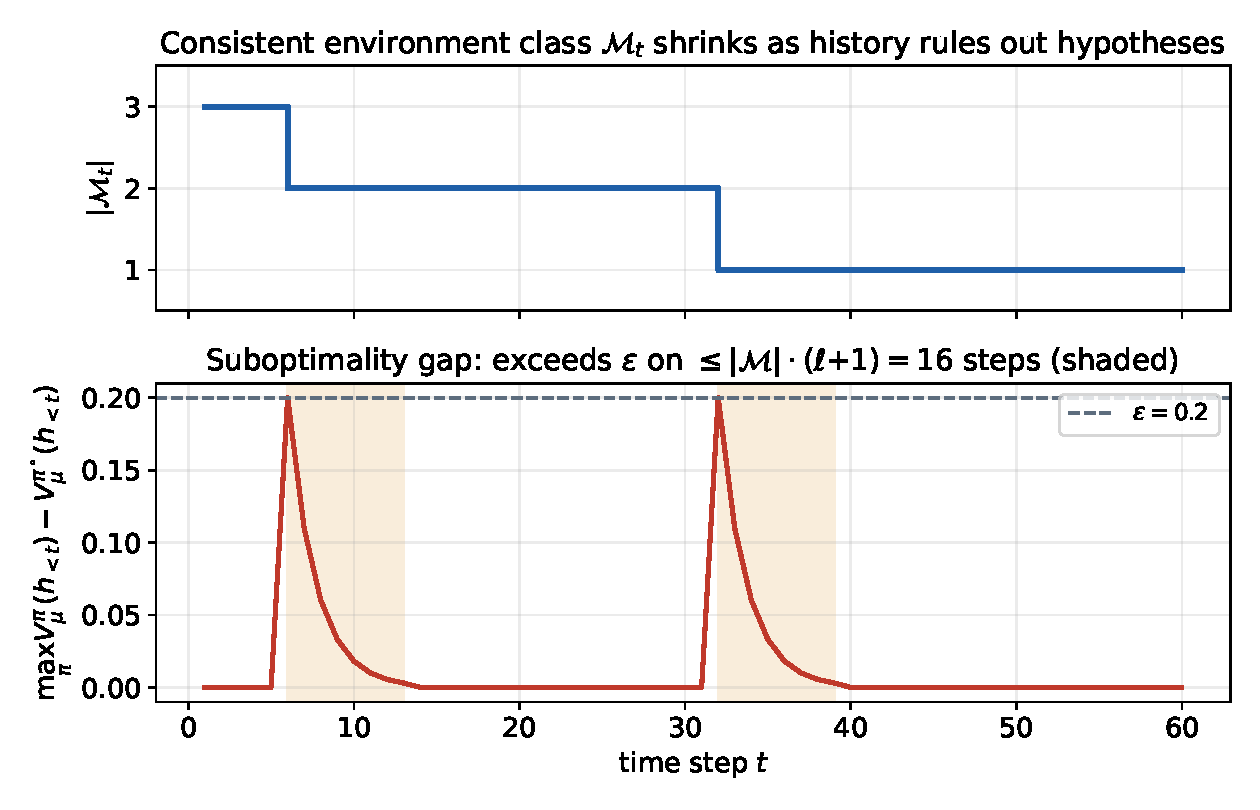
\includegraphics[width=0.62\linewidth]{optimism_bound}
  \end{center}
  {\footnotesize\textbf{Illustration.} Top: $\mathcal{M}_t$ shrinks each
  time an environment is refuted ($3\to2\to1$). Bottom: the suboptimality
  gap exceeds $\varepsilon$ only during the finitely many shaded windows
  right after a refutation. (Synthetic example: $|\mathcal{M}_0|=3$,
  $\gamma=0.8$, $\varepsilon=0.2$, $\ell+1=8$, bound of $16$ bad steps.)}
\end{frame}

\begin{frame}{Algorithm 9.2: Optimistic Agent for Stochastic Environments}
  A similar algorithm handles a \textbf{stochastic} environment class
  $\mathcal{M}_0$. The key difference from Algorithm 9.1 is \emph{how}
  inconsistent environments are removed: a stochastic environment can
  never be refuted with absolute certainty, so we discard any $\nu$ whose
  likelihood of the observed history falls far below (by a factor $z$)
  that of the best-fitting candidate.

  {\small
  \begin{algorithmic}[1]
    \Statex \textbf{Require:} $\mathcal{M}_0=\{\nu_1,\dots,\nu_m\}$. Deterministic policy class $\Pi$
    \Statex \textbf{Require:} Threshold $z\in(0,1)$
    \Statex \textbf{Input:} Value function $V^\pi_\nu$. True environment $\mu$
    \Statex \textbf{Output:} Interaction history $h=a_1e_1a_2e_2a_3e_3\dots$
    \State $t := 1$
    \While{\textbf{True}}
      \State $(\pi^*,\nu^*)\in\arg\max_{\pi\in\Pi,\,\nu\in\mathcal{M}_{t-1}} V^\pi_\nu(h_{<t})$
      \State $a_t := \pi^*(h_{<t})$
      \State Sample $e_t\sim\mu(\cdot\,|\,h_{<t}a_t)$
      \State $h_{1:t} := h_{<t}\,a_t\,e_t$;\quad $t := t+1$
      \State $\mathcal{M}_t := \big\{\nu\in\mathcal{M}_{t-1} : \tfrac{\prod_{j=1}^t \nu(e_j|h_{<j}a_j)}{\max_{\tilde\nu\in\mathcal{M}_0}\prod_{j=1}^t \tilde\nu(e_j|h_{<j}a_j)} > z\big\}$ \Comment{remove inconsistent $\nu$}
    \EndWhile
  \end{algorithmic}}
\end{frame}

\begin{frame}{Algorithm 9.2: Plain-English Summary}
  \textbf{Plain English.} An environment $\nu$ survives only while the
  total probability it assigns to everything observed so far stays within
  a factor $z$ of the best-fitting candidate's probability; falling behind
  means $\nu$ is discarded, even though it was never technically
  ``wrong''.
\end{frame}

\begin{frame}{Theorem 9.1.3: Optimality for Finite Stochastic Classes}
  \begin{block}{Theorem 9.1.3 (Optimality, finite stochastic class [SH12a])}
    Define $\pi^\circ$ via Algorithm 9.2 with any threshold
    $z\in(0,1)$ and a finite class $\mathcal{M}$ of stochastic environments
    containing the true environment $\mu$. Then, with probability at least
    $1-z|\mathcal{M}|$, there exists for every $\varepsilon>0$ a time
    $T<\infty$ such that
    \[
      V^{\pi^\circ}_\mu(h_{<t}) > \max_{\pi\in\Pi} V^\pi_\mu(h_{<t}) - \varepsilon \qquad \forall\, t\ge T
    \]
  \end{block}
  \textbf{Plain English.} With high probability (at least
  $1-z|\mathcal{M}|$ -- close to $1$ if the threshold $z$ is small), the
  optimistic agent again becomes essentially optimal after some finite
  time, this time up to any desired tolerance $\varepsilon$. The proof uses
  martingale theory and is found in [SH12a].
\end{frame}

\begin{frame}{Extending Optimism Beyond Finite Classes}
  \textbf{Extending the idea.} The optimism principle extends further:
  \begin{itemize}
    \item to \textbf{countable} classes $\mathcal{M}$, by running the
      algorithm on a slowly-growing sequence of finite subsets;
    \item to \textbf{compact} classes (w.r.t.\ a metric
      $d(\nu,\nu')=\sup_{h,\pi}|V^\pi_\nu(h)-V^\pi_{\nu'}(h)|$), e.g.\ the
      class of finite-state (Partially Observable) Markov Decision
      Processes, by covering $\mathcal{M}$ with finitely many balls of
      radius $<\varepsilon/2$ and running Algorithm 9.2 on their centres;
    \item further still to \textbf{separable} classes, which can be
      covered by countably many arbitrarily small balls -- but full
      asymptotic optimality (requiring $\varepsilon\to0$) needs the number
      of $\varepsilon$-errors to stay controlled, which for compact subsets
      of $\R^d$ is typically \emph{exponential} in $d$ (the curse of
      dimensionality).
    \item If $\mathcal{M}$ is generated by finite sets of \emph{partial
      environments} (``laws of nature''), error bounds linear in the
      number of laws (rather than the number of environments) are
      possible -- e.g.\ for (PO)MDPs, exponentially improved bounds
      polynomial in $d$ exist.
  \end{itemize}
\end{frame}

\begin{frame}[fragile]{Python: Optimistic Agent on a Toy Deterministic Class}
  We simulate Algorithm 9.1 on $3$ deterministic environments, each defined
  by the fixed observation sequence it emits; the agent rules them out as
  mismatches arrive.
  \begin{lstlisting}[style=pycode]
# Fixed observation sequences the 3 candidate environments emit.
M0 = {"nu1": "0,1,1,0,1", "nu2": "0,1,0,0,1", "nu3": "0,0,1,0,1"}
mu_key = "nu3"                       # nu3 is the TRUE environment

M_t = dict(M0)
true_obs = M0[mu_key].split(",")
for t, e_t in enumerate(true_obs, start=1):
    survivors = {k: v for k, v in M_t.items()
                 if v.split(",")[t - 1] == e_t}
    print(f"t={t} e_t={e_t} |M_t|:{len(M_t)}->{len(survivors)} {list(survivors)}")
    M_t = survivors

# t=1 e_t=0 |M_t|:3->3 ['nu1', 'nu2', 'nu3']
# t=2 e_t=0 |M_t|:3->1 ['nu3']
# t=3 e_t=1 |M_t|:1->1 ['nu3']    (nu3 survives every remaining step)
  \end{lstlisting}
\end{frame}

\begin{frame}{Python Example: What Happened}
  \textbf{What happened.} At $t=2$ the true environment emits observation
  $0$, but $\nu_1$ predicted $1$ -- so $\nu_1$ is discarded immediately.
  From $t=2$ onward only $\nu_3$ (the truth) remains consistent, and by
  Theorem 9.1.1 the agent's policy is then exactly optimal.
\end{frame}

%% ══════════════════════════════════════════════════════════════════════════
\section{9.2 (Thompson) Sampling Agents}

\begin{frame}{The Idea: A Policy That Samples Other Policies}
  Another way to build a policy that performs well is to have a
  \emph{policy which samples from other policies}. A successful version of
  this idea is \textbf{Thompson sampling}, originating with [Tho33] for
  bandit problems and recently rediscovered and applied to reinforcement
  learning and sequential decision theory.

  \vspace{0.4em}
  Like any good Bayesian agent, the Thompson sampler updates its posterior
  at every iteration. But unlike $\mathrm{AI}\xi$, which \emph{mixes} over
  environments (averages them into $\xi$), the Thompson agent \emph{samples}
  a single environment $\nu$ from the posterior distribution and follows
  the policy that is optimal \emph{for that one sampled environment}, for
  an $\varepsilon_t$-effective horizon, then repeats.

  \vspace{0.4em}
  \textbf{Where is the exploration?} It is more subtle than for BayesExp
  (Section 9.4), which explicitly switches between explore/exploit modes.
  In one sense Thompson sampling is \emph{always} exploring, since it never
  commits to the single most likely policy. In another sense, it explores
  precisely when it happens to sample a policy that is not the most likely
  one.
\end{frame}

\begin{frame}{Algorithm 9.3: Thompson Sampling Policy}
  \begin{algorithmic}[1]
    \Statex \textbf{Require:} Model class $\mathcal{M}$. Prior $w$. Effective horizon function $H_t$.
    \Statex \textbf{Input:} Percept stream $e_1,e_2,e_3,\dots$
    \Statex \textbf{Output:} Action stream $a_1,a_2,a_3,\dots$
    \While{\textbf{True}}
      \State sample environment $\nu$ according to the posterior $w(\nu\,|\,h_{<t})$
      \State follow $\pi^*_\nu$ for $H_t(\varepsilon_t)$ time steps
    \EndWhile
  \end{algorithmic}
  \textbf{Plain English.} $H_t(\varepsilon_t)$ is the \textbf{effective
  horizon}: roughly how many future steps still matter given the discount
  function, for tolerance $\varepsilon_t$. So the recipe is: draw one
  hypothesis $\nu$ about the world from your current beliefs, pretend it is
  true, act optimally under that pretence for a while, then draw a fresh
  hypothesis and repeat.

  \vspace{0.4em}
  Note the algorithm glosses over \emph{how} to compute the posterior
  $w(\nu|h_{<t})$ and the $\nu$-optimal policy $\pi^*_\nu$ -- for the
  largest class $\mathcal{M}_{\mathrm{sol}}$ of all computable environments
  this is exactly as hard as computing $\pi^*_\xi$ itself, but it may be
  much simpler for restricted classes, e.g.\ when $\mathcal{M}$ is a
  (sub)class of MDPs.
\end{frame}

\begin{frame}{Theorem 9.2.1 \& Corollary 9.2.2}
  \begin{block}{Theorem 9.2.1 (Thompson sampling is asymptotically optimal in mean [Lei16b])}
    For all $\mu\in\mathcal{M}$, for the Thompson sampling agent
    $\pi_{\mathrm{TS}}$, we have
    \[
      \E^{\pi_{\mathrm{TS}}}_\mu\big[V^*_\mu(h_{<t}) - V^{\pi_{\mathrm{TS}}}_\mu(h_{<t})\big] \to 0 \qquad \text{for } t\to\infty
    \]
  \end{block}
  \textbf{Plain English.} $\E$ denotes \textbf{expectation} (an average over
  randomness). This says that, \emph{on average}, the gap between the best
  possible value $V^*_\mu$ and Thompson sampling's actual value shrinks to
  zero as time goes on -- the agent is optimal ``in mean''. This is weaker
  than being optimal on \emph{every} run (Definition 8.1.7, strong
  asymptotic optimality) -- indeed $\pi_{\mathrm{TS}}$ is \emph{not} strongly
  asymptotically optimal, though it does converge in probability too.
\end{frame}

\begin{frame}{Corollary 9.2.2: Sublinear Regret}
  \begin{block}{Corollary 9.2.2 (Sublinear regret for Thompson sampling [Lei16b])}
    If the discount function $\gamma$ satisfies Assumption 8.1.11, and the
    environment $\mu\in\mathcal{M}$ is recoverable, then the regret is
    sublinear: $\mathrm{Regret}_m(\pi_{\mathrm{TS}},\mu) = o(m)$.
  \end{block}
  \textbf{Plain English.} \textbf{Regret} measures the total reward lost
  (over $m$ steps) compared to always acting optimally. ``Sublinear'' means
  regret grows strictly slower than $m$ itself, so the \emph{average}
  per-step regret vanishes -- a standard, strong notion of learning
  efficiency. \textbf{Recoverable} environments are ones where mistakes do
  not permanently destroy the chance of eventually acting well.
\end{frame}

\begin{frame}[fragile]{Python: Thompson Sampling on a Toy 3-Environment Class}
  We simulate Thompson sampling on a Bernoulli bandit with $3$ candidate
  environments $\nu_1,\nu_2,\nu_3$ with unknown success probabilities
  $0.3,0.5,0.8$; the true environment is $\nu_3$. The posterior over each
  $\nu_i$'s success probability is tracked with a Beta distribution
  (the standard conjugate posterior for Bernoulli observations).
  \begin{lstlisting}[style=pycode]
import numpy as np
rng = np.random.default_rng(7)

true_p   = np.array([0.30, 0.50, 0.80])   # nu_1, nu_2, nu_3
alpha, beta = np.ones(3), np.ones(3)      # uniform Beta(1,1) priors

for t in range(300):
    sample = rng.beta(alpha, beta)        # draw one nu per candidate
    a = int(np.argmax(sample))            # nu with highest sampled p
    r = rng.binomial(1, true_p[a])        # follow pi*_nu, observe reward
    alpha[a] += r; beta[a] += (1 - r)     # Bayesian posterior update

print("posterior means:", alpha / (alpha + beta))
# -> posterior means: [0.29 0.45 0.76]   (close to true_p, nu_3 favoured)
  \end{lstlisting}
\end{frame}

\begin{frame}{Thompson Sampling: Posterior Convergence}
  \begin{center}
    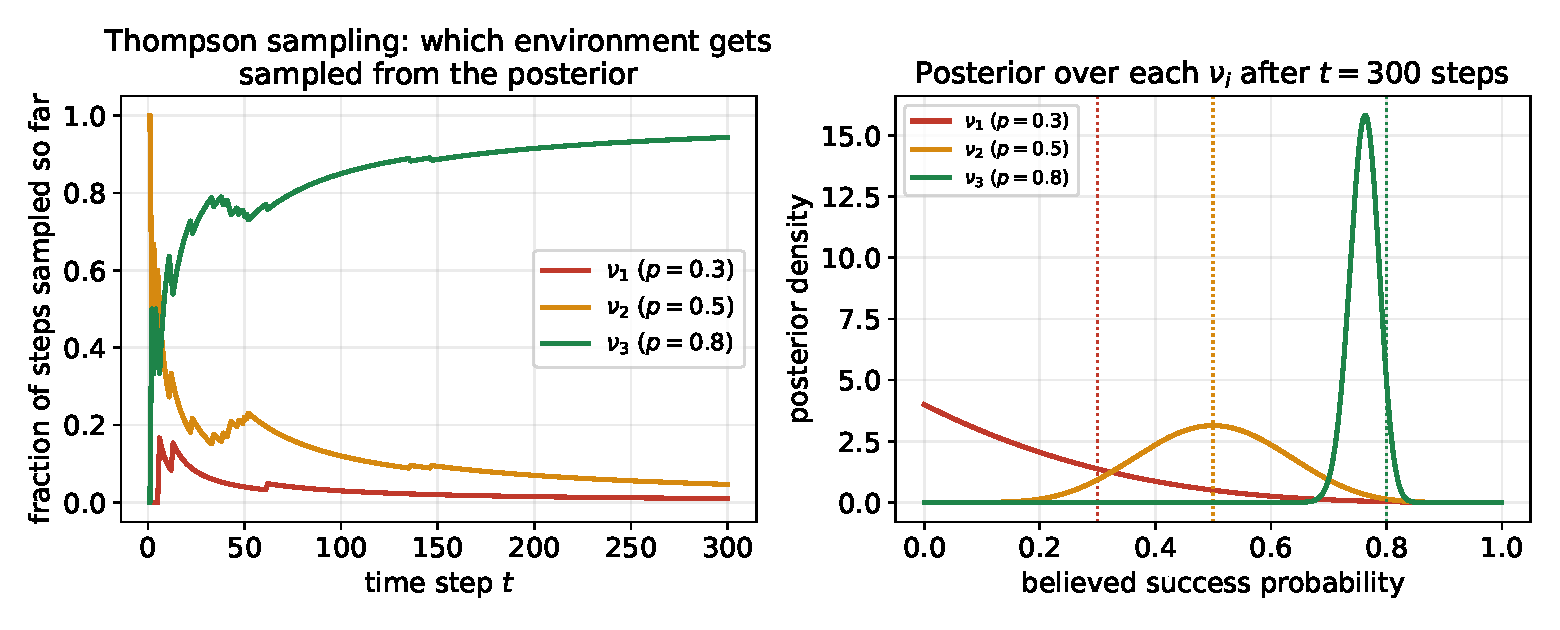
\includegraphics[width=0.7\linewidth]{thompson_sampling}
  \end{center}
  \textbf{Left:} the fraction of time steps in which each environment gets
  sampled converges to always picking the true best one, $\nu_3$.
  \textbf{Right:} after $300$ steps, the posterior densities have sharpened
  around each environment's true success probability (dotted lines).
\end{frame}

%% ══════════════════════════════════════════════════════════════════════════
\section{9.3 Knowledge-Seeking Agents}

\begin{frame}{Motivation: What Should an Agent Without Rewards Want?}
  One of the fundamental questions in defining general intelligence is:
  where should rewards come from? Any reward provided by humans is
  susceptible to \textbf{manipulation} (discussed in Chapter 15) -- and it
  is unclear to what degree an agent that simply maximizes externally
  supplied reward is autonomously intelligent at all. A reward function
  should not be tied to a specific goal (winning chess, driving from $A$
  to $B$), but should instead encourage \emph{general} competence.

  \vspace{0.4em}
  A reward function based purely on \emph{how much the agent has learned}
  seems both general and useful. Agents built this way are called
  \textbf{curiosity-driven agents} [Sch91] or \textbf{Knowledge-Seeking
  Agents} (KSA). Seeking out information encourages exploration, which
  allows the agent to learn and solve problems.

  \vspace{0.4em}
  We measure \textbf{Information Gain (IG)} using the \textbf{KL
  divergence} (Kullback--Leibler divergence, a standard measure of how
  different two probability distributions are; Definition 2.5.12) as a
  replacement for reward. Other distance measures exist, but most perform
  poorly in stochastic environments, chasing noise instead of genuine
  novelty [OLH13].
\end{frame}

\begin{frame}{Definition 9.3.1: Information Gain}
  \begin{block}{Definition 9.3.1 (Information Gain)}
    The one-step information gain of $h_k\in\mathcal{A}\times\mathcal{E}$
    given history $h_{<k}\in(\mathcal{A}\times\mathcal{E})^{k-1}$ is defined
    as the KL divergence between the posterior conditioned on history
    $h_{1:k}$, and the posterior given history $h_{<k}$:
    \[
      r_k^{\IG} \;:=\; \IG(h_k\,|\,h_{<k}) \;:=\; \sum_{\nu\in\mathcal{M}} w(\nu|h_{1:k})\, \log\frac{w(\nu|h_{1:k})}{w(\nu|h_{<k})}
    \]
  \end{block}
  \textbf{Plain English.} $\mathcal{A}\times\mathcal{E}$ is the space of
  action-percept pairs; $h_k$ is the single action-percept pair observed at
  time $k$. $\IG(h_k|h_{<k})$ measures how much the posterior belief
  \emph{changed} after seeing $h_k$: if $h_k$ was very surprising (the
  posterior $w(\cdot|h_{<k})$ assigned it very low probability), the belief
  shifts a lot and the KL divergence -- hence the information gain -- is
  large. If the agent's belief was already accurate
  ($w(\mu|h_{<k})\approx1$), it only observes what it expected anyway, so
  $w(\cdot|h_{1:k})\approx w(\cdot|h_{<k})$ and the information gain is
  small.

  \vspace{0.3em}
  This one-step definition extends naturally to an arbitrary (finite)
  history window $h_{k:k+\ell}$ instead of a single pair $h_k$; we mainly
  use the one-step version, replacing the ordinary reward $r_k$ in the
  usual value function (Definition 6.6.1) with the information-gain
  ``reward'' $r_k^{\IG}$.
\end{frame}

\begin{frame}{Definition 9.3.2: Information Gain Value Function}
  \begin{block}{Definition 9.3.2 (Information Gain Value function)}
    The information gain value of policy $\pi$ having observed history
    $h_{<t}$ with respect to discount function $\gamma$, denoted
    $V^{\pi,m}_{\IG}$, is the $\xi$-expected discounted information gain:
    \[
      V^{\pi,m}_{\IG}(h_{<t}) \;:=\; \E^\pi_\xi\Big[\,\frac{1}{\Gamma_t}\sum_{k=t}^{m}\gamma_k\,\IG(h_k|h_{<k})\ \Big|\ h_{<t}\Big]
    \]
    (we drop $m$ when $m=\infty$). The \textbf{optimal information gain
    policy} $\pi^*_{\IG}$ maximizes this value function:
    \[
      \pi^*_{\IG}(\cdot) :\in \arg\max_\pi V^\pi_{\IG}(\cdot) \qquad\text{and}\qquad V^*_{\IG}(\cdot) := \max_\pi V^\pi_{\IG}(\cdot)
    \]
  \end{block}
  \textbf{Plain English.} This is exactly the ordinary value function
  machinery from Chapter 6, but with the reward at each step replaced by
  the information gain at that step. The KSA policy $\pi^*_{\IG}$ is simply
  the policy that maximizes expected total (discounted) information gain
  -- it seeks out actions likely to be the most surprising/informative,
  rather than the most rewarding.
\end{frame}

\begin{frame}{Definition 9.3.3: KL-Divergence for $\nu^\pi$ and $\xi^\pi$}
  Information gain measures distance between successive \emph{posteriors}.
  A related and useful quantity measures the distance between the
  \textbf{predictive policy-environment distributions} $\nu^\pi$ (what
  policy $\pi$ predicts will happen if $\nu$ is the true environment) and
  $\xi^\pi$ (what $\pi$ predicts under the Bayes mixture).

  \begin{block}{Definition 9.3.3 (KL-Divergence for $\nu^\pi$ and $\xi^\pi$)}
    Given a history $h_{<k}$, the one-step KL divergence between
    $\nu^\pi$ and $\xi^\pi$ is
    \[
      \tilde r_k^{\,\nu} \;:=\; \mathrm{KL}_1(\nu^\pi,\xi^\pi|h_{<k}) \;:=\; \sum_{h_k\in\mathcal{A}\times\mathcal{E}} \nu^\pi(h_k|h_{<k})\, \log\frac{\nu^\pi(h_k|h_{<k})}{\xi^\pi(h_k|h_{<k})}
    \]
  \end{block}
  \textbf{Plain English.} Unlike $r_k^{\IG}$, this quantity $\tilde r_k^\nu$
  depends explicitly on $\nu$ and therefore \emph{cannot} literally be used
  as a reward (the agent does not know the true $\nu$) -- but it is a
  valuable theoretical device, because (Equation 9.3.4) the corresponding
  $\nu$-value function
  \[
    \tilde V^{\pi,m}_{\nu,\gamma}(h_{<t}) \;\equiv\; \frac{1}{\Gamma_t}\E^\pi_\nu\Big[\sum_{k=t}^m \gamma_k\tilde r_k^{\,\nu}\ \Big|\ h_{<t}\Big]
    \;\equiv\; \frac{1}{\Gamma_t}\sum_{k=t}^m\gamma_k\sum_{h_{t:k-1}} \nu^\pi(h_{t:k-1}|h_{<t})\,\mathrm{KL}_1(\nu^\pi,\xi^\pi|h_{<k})
  \]
  lets us relate information gain (an agent-observable quantity) directly
  to the KL divergence between the true dynamics $\nu^\pi$ and the agent's
  believed dynamics $\xi^\pi$ (a quantity about learning accuracy).
\end{frame}

\begin{frame}{Lemma 9.3.5: Information Gain in Terms of KL Divergence}
  \begin{block}{Lemma 9.3.5 (Information gain in terms of KL divergence)}
    The information gain value function can be expressed via the KL
    divergence between two policy-environment distributions:
    \[
      V^{\pi,m}_{\IG}(h_{<t}) \;=\; \sum_{\nu\in\mathcal{M}} w(\nu|h_{<t})\,\tilde V^{\pi,m}_{\nu,\gamma}(h_{<t})
    \]
  \end{block}
  \textbf{Plain English.} This is the crucial bridge result: the
  information-gain value that the agent can actually compute and optimize
  (left-hand side) equals a posterior-weighted average, over every
  candidate environment $\nu$, of how far the agent's beliefs currently are
  from that particular candidate's true dynamics (right-hand side). Chasing
  information gain is therefore mathematically the same as chasing
  accuracy about the (weighted) truth.

  \vspace{0.4em}
  \textbf{Proof outline.} Expanding the definitions of $V_{\IG}$ and $\IG$,
  pushing the sum over full histories $h_{t:m}$ inward so it cancels against
  the mixture normalization ($\sum_{h_{k:m}}\xi^\pi(h_{k:m}|h_{<t})=1$),
  rewriting $\nu(e_t|h_{<t}a_t)/\xi(e_t|h_{<t}a_t)$ using Definition 7.2.2 of
  the posterior, splitting $\nu^\pi(h_{t:k}|h_{<t})$ into a product over the
  step $k$, and finally recognizing Definition 9.3.3's KL divergence and
  substituting Equation 9.3.4, telescopes exactly into the claimed identity.
  $\blacksquare$
\end{frame}

\begin{frame}{Theorem 9.3.6: On-Policy Prediction}
  \begin{block}{Theorem 9.3.6 (On-policy prediction [OLH13])}
    Let $\mu\in\mathcal{M}$ and $\pi$ be a policy, and
    $\sum_{\nu\in\mathcal{M}} w_\nu\log w_\nu^{-1}<\infty$, then
    \[
      \E^\pi_\mu\big[\tilde V^\pi_\mu(h_{<t})\big] \;\xrightarrow{t\to\infty}\; 0
    \]
  \end{block}
  \textbf{Plain English.} The finiteness condition
  $\sum_\nu w_\nu\log w_\nu^{-1}<\infty$ says the prior's \textbf{entropy}
  is finite (roughly: the prior does not spread belief \emph{too} thinly
  over too many hypotheses). Under that condition, this theorem shows that
  the mixture's on-policy predictions $\mathrm{P}^\pi_\xi(\cdot|h_{<t})$
  converge (in expectation, measured via cumulative discounted KL
  divergence) to the true predictions $\mathrm{P}^\pi_\mu(\cdot|h_{<t})$.
  In other words, $\xi$ becomes, in expectation, a good estimate of the
  unknown true predictive distribution -- \emph{as long as the agent keeps
  following policy $\pi$} (this is why it's called \emph{on-policy}).

  \vspace{0.3em}
  The finite-entropy condition fails for our usual canonical prior
  $w_\nu^U = 2^{-K(\nu)}$ on $\mathcal{M}_{\mathrm{sol}}$ ($K(\nu)$ is the
  Kolmogorov complexity of $\nu$ -- its shortest description length), but
  is easily satisfied by a marginally faster-decaying prior, e.g.\
  $w_\nu = 2^{-(1+\varepsilon)K(\nu)}$, or $w_\nu = 2^{-K(\nu)}/K(\nu)$, or
  $w_{\nu_i}=1/(i+1)^2$ (Exercise 7).
\end{frame}

\begin{frame}[allowframebreaks]{Proof of Theorem 9.3.6}
  The telescoping property of KL divergence (lifted to our setting, as in
  Lemma 3.2.4) gives
  \begin{align}
    \E^\pi_\nu\Big[\sum_{k=t}^m \mathrm{KL}_1(\nu^\pi,\xi^\pi|h_{<t})\Big]
      &\equiv \E^\pi_\nu\Big[\sum_{k=1}^m\mathrm{KL}_1(\nu^\pi,\xi^\pi|h_{<t}) - \sum_{k=1}^{t-1}\mathrm{KL}_1(\nu^\pi,\xi^\pi|h_{<t})\Big] \notag\\
      &= \mathrm{KL}(\nu^\pi_{1:m}\|\xi^\pi_{1:m}) - \mathrm{KL}(\nu^\pi_{<t}\|\xi^\pi_{<t}) \tag{9.3.7}
  \end{align}
  As a sum of non-negative terms, $\mathrm{KL}(\nu^\pi_{1:m}\|\xi^\pi_{1:m})$
  is increasing in $m$ and converges to $c^\xi_\nu\le\log w_\nu^{-1}<\infty$,
  by \textbf{dominance} $\xi^\pi\ge w_\nu\nu^\pi$ (Lemma 7.2.4: the mixture
  is always at least $w_\nu$ times any single constituent). Hence
  \[
    \lim_{t\to\infty}\E^\pi_\nu\Big[\sum_{k=t}^\infty \mathrm{KL}_1(\nu,\xi|h_{<t})\Big] = c^\xi_\nu - c^\xi_\nu = 0. \tag{9.3.8}
  \]

  \framebreak
  Also, using the positivity of KL divergence to introduce the missing sum
  over $\nu$ (a), and $\gamma_k/\Gamma_t\le1$ for $k\ge t$ together with
  the tower rule $\E[\E[\cdot|h_t]]=\E[\cdot]$ (b),
  \[
    \E^\pi_\mu\big[\tilde V^\pi_\mu(h_{<t})\big]
      \;\overset{(a)}{\le}\; \frac{1}{w_\mu}\sum_{\nu\in\mathcal{M}} w_\nu \E^\pi_\nu\Big[\sum_{k=t}^\infty \tilde V^\pi_\nu(h_{<t})\Big]
      \;\overset{(b)}{\le}\; \frac{1}{w_\mu}\sum_{\nu\in\mathcal{M}} w_\nu \E^\pi_\nu\Big[\sum_{k=t}^\infty \tilde r_k^{\,\nu}\Big] \tag{9.3.9}
  \]
  Define $\delta_\nu(t):=\E^\pi_\nu\big[\sum_{k=t}^\infty \tilde r_k^{\,\nu}\big]\to0$, which follows from Definition 9.3.3 and (9.3.8).

  \framebreak
  We also know $\delta_\nu(t)\le\mathrm{KL}(\nu^\pi\|\xi^\pi)\le\log w_\nu^{-1}$
  from (9.3.7) and dominance. Unfortunately $\delta_\nu(t)$ is not
  \emph{uniformly} bounded across $\nu$, so we cannot directly conclude
  $\sum_\nu w_\nu\delta_\nu(t)\to0$ (a lemma from [Hut05b] needs uniform
  boundedness). The fix: define
  $\tilde w_\nu := w_\nu\log w_\nu^{-1} > 0$ and
  $\tilde\delta_\nu(t) := \delta_\nu(t)/\log w_\nu^{-1} \le 1$. By our
  finite-entropy assumption, $\sum_\nu\tilde w_\nu<\infty$, so now the
  lemma \emph{does} apply to these ``tilded'' quantities, giving
  \[
    0 \;\le\; \E^\pi_\mu\big[\tilde V^\pi_\mu(h_{<t})\big] \;\le\; \frac{1}{w_\mu}\sum_\nu \tilde w_\nu\tilde\delta_\nu(t) \;\xrightarrow{t\to\infty}\; 0. \qquad\blacksquare
  \]
\end{frame}

\begin{frame}{Theorem 9.3.10: On-Policy Learning, Off-Policy Prediction}
  The next result is perhaps the most important theoretical justification
  for defining $\pi^*_{\IG}$ at all. It shows that if the agent's history
  $h_{1:\infty}$ is generated by \emph{following} $\pi^*_{\IG}$, then
  $\mathrm{P}^\pi_\xi(\cdot|h_{<t})$ converges in expectation to
  $\mathrm{P}^\pi_\mu(\cdot|h_{<t})$ for \emph{every} policy $\pi$ -- not
  just the one being followed. Informally: the longer the agent explores
  by chasing information, the better it can predict the counterfactual
  ``what would happen if I followed policy $\pi$ instead''.

  \begin{block}{Theorem 9.3.10 (On-policy learning, off-policy prediction [Ors11])}
    Let $\mu\in\mathcal{M}$ and $\sum_{\nu\in\mathcal{M}} w_\nu\log w_\nu^{-1}<\infty$. Then
    \[
      \E^{\pi^*_{\IG}}_\mu\Big[\sup_\pi \tilde V^\pi_\mu(h_{<t})\Big] \;\xrightarrow{t\to\infty}\; 0
    \]
    where the expectation is taken over $h_{<t}$.
  \end{block}
  \textbf{Plain English.} If the observation stream also included a reward
  signal, this off-policy prediction ability means the agent would
  asymptotically be able to \emph{learn} (though not necessarily
  \emph{follow}) the policy that maximizes expected discounted reward --
  the policy maximizing Bayes-expected reward would converge to optimal.
  Most policies only achieve the weaker on-policy guarantee of Theorem
  9.3.6; achieving off-policy prediction is special to $\pi^*_{\IG}$.
\end{frame}

\begin{frame}{Proof of Theorem 9.3.10}
  By positivity of KL divergence (adding non-negative
  $\tilde V^\pi_\nu(h_{<t})\ge0$ terms for all $\nu$), then Lemma 9.3.5 and
  the definition of $\pi^*_{\IG}$ as the maximizer of $V_{\IG}$:
  {\small
  \[
    \E^{\pi^*_{\IG}}_\mu\Big[\sup_\pi\tilde V^\pi_\mu(h_{<t})\Big]
    \;\le\; \E^{\pi^*_{\IG}}_\mu\Big[\tfrac{1}{w(\mu|h_{<t})}\sup_\pi\textstyle\sum_{\nu\in\mathcal{M}} w(\nu|h_{<t})\tilde V^\pi_\nu(h_{<t})\Big]
  \]
  \[
    \;=\; \E^{\pi^*_{\IG}}_\mu\Big[\tfrac{1}{w(\mu|h_{<t})}\textstyle\sum_{\nu\in\mathcal{M}} w(\nu|h_{<t})\tilde V^{\pi^*_{\IG}}_\nu(h_{<t})\Big]
  \]}
  From the definition of the posterior and expectation, then exchanging
  the sum and expectation and using the definition of the posterior again:
  {\small
  \[
    = \frac{1}{w_\mu}\E^{\pi^*_{\IG}}_\xi\Big[\sum_{\nu\in\mathcal{M}} w(\nu|h_{<t})\tilde V^{\pi^*_{\IG}}_\nu(h_{<t})\Big]
    = \frac{1}{w_\mu}\sum_{\nu\in\mathcal{M}} w_\nu\, \E^{\pi^*_{\IG}}_\nu\big[\tilde V^{\pi^*_{\IG}}_\nu(h_{<t})\big] \;\xrightarrow{t\to\infty}\; 0
  \]}
  The limit follows from (9.3.9), choosing $\pi=\pi^*_{\IG}$. $\blacksquare$
\end{frame}

\begin{frame}{Knowledge-Seeking Agents: Takeaway}
  \textbf{Takeaway.} Knowledge-seeking agents aim to maximize value with
  respect to Bayesian mixtures over environments, and so share the same
  properties as Bayes-optimal agents: they depend on the choice of prior
  and can behave suboptimally in the short term. However, because KSAs
  continuously learn \emph{off-policy} and are asymptotically optimal
  \textbf{without any recoverability assumption} (unlike Thompson
  sampling), the choice of prior ultimately does not affect long-run
  performance.
\end{frame}

\begin{frame}{Example 9.3.11: KSA Experiments on Toy Environments}
  Consider the KL-KSA agent with a (deterministic) environment model class
  $\mathcal{M}=\{\mu_1,\mu_2,\mu_3\}$ given by the state diagrams below. All
  three environments are identical except for slight differences in the
  transitions highlighted in \textbf{bold}. State $q_1$ is a \textbf{trap
  state}: once visited, the agent can never leave.

  \begin{center}
    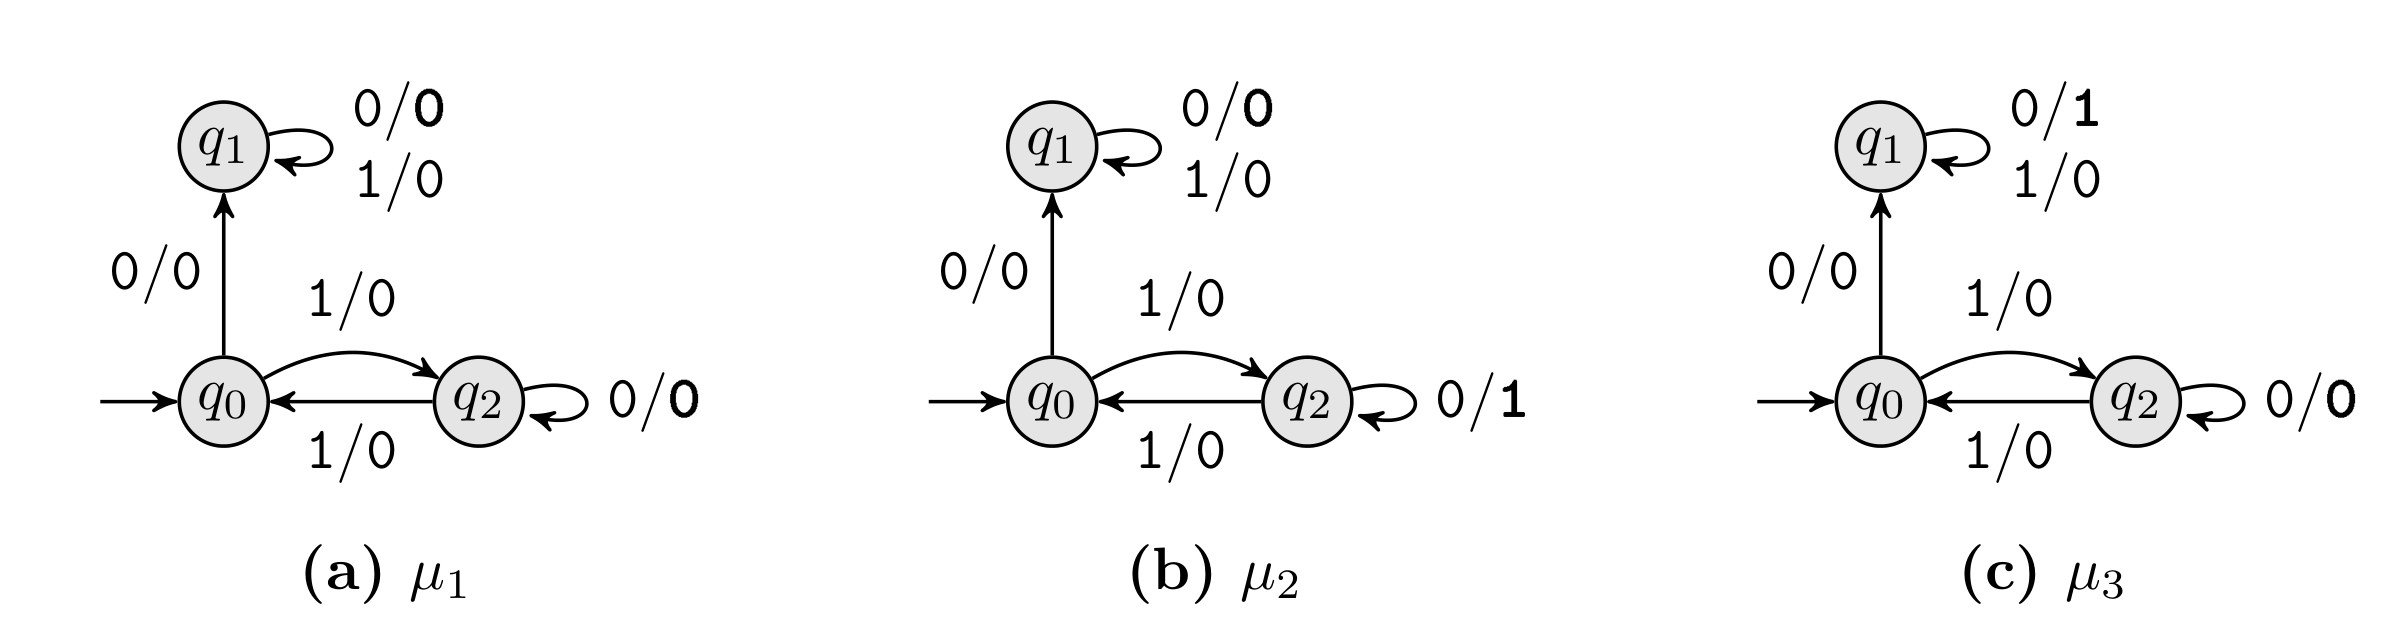
\includegraphics[width=0.95\linewidth]{toy_environments}
  \end{center}
  From $q_0$, action $1$ moves to $q_2$ and back (obs.\ always $0$); action
  $0$ from $q_0$ moves permanently into the trap $q_1$ (obs.\ $0$). The
  only place the three environments differ is what the self-loop
  observation is at $q_1$ under action $0$ (environment $\mu_3$ emits $1$
  instead of $0$) and at $q_2$ under action $0$ (environment $\mu_2$ emits
  $1$ instead of $0$).
\end{frame}

\begin{frame}{Example 9.3.11, Continued: The Optimal Exploration Sequence}
  To learn the true environment as fast as possible, the agent should take
  actions $\dot a_{1:5}=\texttt{10100}$ and receive a sequence of
  observations $o'_{1:5}$ depending on the true environment: either
  \texttt{00000} for $\mu_1$, \texttt{01000} for $\mu_2$, or \texttt{00001}
  for $\mu_3$. \textbf{No other} action sequence can distinguish with
  certainty between the three environments in strictly fewer time steps.

  \vspace{0.4em}
  Also, if the agent chooses $a_1=0$, it is stuck in the trap state
  forever, and can \emph{never} distinguish $\mu_1$ from $\mu_2$ (if either
  is the true environment) -- both produce identical observations at $q_1$
  under action $0$.

  \vspace{0.4em}
  Of all possible action sequences $a_{1:\infty}$, the KSA agent values
  those prefixed with $\dot a_{1:5}=\texttt{10100}$ the \emph{highest},
  indicating that it learns as fast as possible for this toy model class,
  and avoids moving into the trap state while there is still information
  to learn elsewhere.
\end{frame}

\begin{frame}{Example 9.3.11: Ranking Action Prefixes by Information Gain}
  \begin{center}
    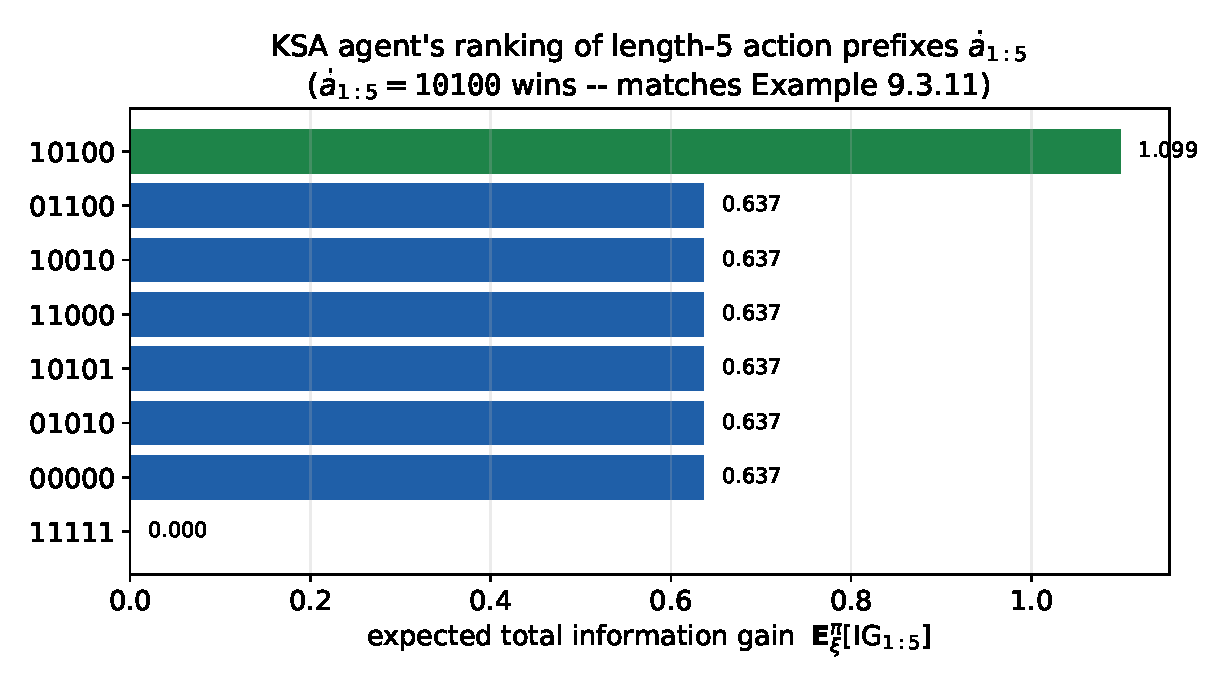
\includegraphics[width=0.85\linewidth]{ksa_infogain}
  \end{center}
\end{frame}

\begin{frame}[fragile]{Python: Recreating Example 9.3.11 (1/2 -- the Automaton)}
  We simulate the exact automaton from Figure 9.1: each candidate
  environment differs only in what it observes at the self-loops of $q_1$
  and $q_2$ under action $0$.
  \begin{lstlisting}[style=pycode]
def step(state, action, env):           # env in {1,2,3}; Figure 9.1
    obs_q1_a0 = {1: 0, 2: 0, 3: 1}[env]  # self-loop obs. at trap q1
    obs_q2_a0 = {1: 0, 2: 1, 3: 0}[env]  # self-loop obs. at q2
    if state == "q0":
        return ("q1", 0) if action == 0 else ("q2", 0)
    if state == "q1":
        return ("q1", obs_q1_a0 if action == 0 else 0)
    return ("q2", obs_q2_a0) if action == 0 else ("q0", 0)

def obs_sequence(actions, env):
    s, out = "q0", []
    for a in actions:
        s, o = step(s, a, env)
        out.append(o)
    return tuple(out)
  \end{lstlisting}
\end{frame}

\begin{frame}[fragile]{Python: Recreating Example 9.3.11 (2/2 -- Information Gain)}
  Now compute the expected total information gain, Definitions
  9.3.1--9.3.2 (undiscounted, over $5$ steps, uniform prior $\tfrac13$ over
  $\mu_1,\mu_2,\mu_3$), for several candidate $5$-action prefixes.
  \begin{lstlisting}[style=pycode]
def expected_info_gain(actions, envs=(1, 2, 3)):
    obs = {e: obs_sequence(actions, e) for e in envs}
    total = 0.0
    for true_env in envs:                      # average over which env is true
        w = {e: 1/3 for e in envs}
        for k in range(len(actions)):
            w_new = {e: (w[e] if obs[e][:k+1] == obs[true_env][:k+1] else 0.0)
                     for e in envs}
            z = sum(w_new.values()); w_new = {e: v/z for e, v in w_new.items()}
            for e in envs:
                if w_new[e] > 0 and w[e] > 0:
                    total += (1/3) * w_new[e] * __import__("math").log(w_new[e]/w[e])
            w = w_new
    return total

for a in ["10100", "00000", "11111"]:
    print(a, "->", round(expected_info_gain([int(c) for c in a]), 3))
# 10100 -> 1.099   (= log 3: fully distinguishes all three environments)
# 00000 -> 0.637   (stuck in trap; only rules mu_3 in/out, never mu_1 vs mu_2)
# 11111 -> 0.0     (never takes action 0; observations identical for all env)
  \end{lstlisting}
\end{frame}

%% ══════════════════════════════════════════════════════════════════════════
\section{9.4 Exploring Agents (BayesExp and Inq)}

\begin{frame}{The Exploration--Exploitation Problem}
  While acting in an environment, we often want the agent to explore
  enough that an optimal action can eventually be identified. How much
  time should the agent spend exploring? Exploring too much means the
  agent never acts optimally, only ever taking novel actions. Exploring
  too little means the agent prematurely commits to an action based on an
  inaccurate model. This trade-off is the classic
  \textbf{exploration--exploitation problem}.

  \vspace{0.4em}
  Unexpectedly, the Bayes-optimal agent $\mathrm{AI}\xi$ does \emph{not}
  explore enough to be asymptotically optimal (Theorem 8.3.1) -- but this
  can be fixed by adding ``a bit'' of extra, deliberate exploration, though
  it is not obvious \emph{whether} we should always want to [CHC21].
\end{frame}

\begin{frame}{Algorithm 9.4: BayesExp}
  Under reasonable assumptions, there exists an agent that balances
  exploration and exploitation to achieve (weak) asymptotic optimality:
  \textbf{BayesExp}, a Bayesian agent with extra exploration, switches
  between exploring and exploiting in just the right way that asymptotically
  the exploiting phase becomes optimal -- though there is always a non-zero
  chance of exploring.

  {\small
  \begin{algorithmic}[1]
    \Statex \textbf{Require:} Non-increasing sequence $\varepsilon_1,\varepsilon_2,\varepsilon_3,\dots$
    \Statex \textbf{Require:} Model class $\mathcal{M}$. Prior $w$. Effective horizon function $H_t(\cdot)$.
    \Statex \textbf{Input:} Percept stream $e_1,e_2,e_3,\dots$
    \Statex \textbf{Output:} Action stream $a_1,a_2,a_3,\dots$
    \While{\textbf{True}}
      \If{$V^{*,\,t+H_t(\varepsilon_t)}_{\IG}(h_{<t}) > \varepsilon_t$}
        \State follow $\pi^*_{\IG}$ for $H_t(\varepsilon_t)$ steps \Comment{exploration}
      \Else
        \State follow $\pi^*_\xi$ for $1$ step \Comment{exploitation}
      \EndIf
    \EndWhile
  \end{algorithmic}}
\end{frame}

\begin{frame}{Algorithm 9.4: Plain-English Summary}
  \textbf{Plain English.} At each decision point, BayesExp checks whether
  the \emph{best achievable} expected information gain over the next
  $H_t(\varepsilon_t)$ steps exceeds the current threshold $\varepsilon_t$.
  If yes, it commits to exploring (following the knowledge-seeking policy
  $\pi^*_{\IG}$) for that whole block of steps. If not, it takes a single
  Bayes-optimal exploitation step and re-checks.
\end{frame}

\begin{frame}{Theorem 9.4.1: BayesExp Is Weakly Asymptotically Optimal}
  \begin{block}{Theorem 9.4.1 (BayesExp is weakly asymptotically optimal [Lat14])}
    Let $\mathcal{M}=\{\nu_1,\nu_2,\dots\}$ be countable and
    $\sum_{\nu\in\mathcal{M}} w_\nu\log w_\nu^{-1}<\infty$, and discount
    $\gamma_t$ and exploration thresholds $\varepsilon_t$ satisfying
    \begin{itemize}
      \item $\Gamma_t>0$ for all $t$
      \item $H_{t+1}(\varepsilon)\ge H_t(\varepsilon)$, for all
        $\varepsilon>0$ and all $t\in\N$
      \item $\varepsilon_{t+1}\le\varepsilon_t$ for all $t$
      \item $\lim_{t\to\infty}\varepsilon_t=0$
      \item $H_t(\varepsilon_t)=o(t\varepsilon_t)$
    \end{itemize}
    Then BayesExp is weakly asymptotically optimal in $(\mathcal{M},\gamma)$.
  \end{block}
  \textbf{Plain English.} These conditions just say: the effective horizon
  doesn't shrink over time, the exploration threshold decreases (but not
  instantly to zero), and the total time spent exploring
  ($H_t(\varepsilon_t)$) grows strictly slower than $t\varepsilon_t$. Given
  all that, BayesExp achieves \textbf{weak asymptotic optimality}
  (Definition 8.1.5: optimal on average / in the limit of Cesàro averages).
\end{frame}

\begin{frame}{Proof Idea for Theorem 9.4.1}
  \textbf{Proof idea [Lat14].} (i) $\pi^*_\xi$ converges to the truly
  optimal $\pi^*_\mu$ on BayesExp's exploitation steps; (ii) the number of
  exploration steps taken is $o(n)$ (a vanishing fraction of total time);
  (iii) the value of $\pi_{\mathrm{BE}}$ converges to the value of
  $\pi^*_\xi$ in Cesàro average. Together these imply weak asymptotic
  optimality. $\blacksquare$
\end{frame}

\begin{frame}{Why BayesExp Works}
  BayesExp's ability to balance exploration and exploitation stems from its
  \emph{dynamic} exploration strategy: it adjusts the number of exploration
  steps based on the maximum expected information gain and a predefined
  threshold.

  \begin{itemize}
    \item As the agent progresses, the threshold $\varepsilon_t$ decreases
      toward $0$, ensuring BayesExp keeps exploring \emph{as long as}
      information can still be gained.
    \item At the same time, $\varepsilon_t\to0$ \emph{slowly enough} that
      the probability of exploration also tends to $0$ overall -- this
      gradual transition is what makes the trade-off work.
    \item One can show that for \emph{any} discount with a monotonically
      but sublinearly growing effective horizon, a valid exploration
      sequence $\varepsilon_t$ exists (Exercise 4); e.g.\ geometric
      discount $\gamma_t=\gamma^t$ has constant effective horizon, and
      $\varepsilon_t=t^{-\beta}$ ($\beta$ (beta), any $0<\beta<1$) works.
  \end{itemize}
\end{frame}

\begin{frame}{Why BayesExp Works, Continued}
  \begin{itemize}
    \item For deterministic environments and geometric discounting, the
      proof is much simpler (environments can be ruled out completely, as
      in Section 9.1); the stochastic-case proof is beyond the scope of
      the book [Lat14].
    \item Since $\varepsilon_t\to0$, at exploitation time-steps the
      expected information gain converges to $0$, meaning $\xi$
      concentrates around $\mu$ while exploiting -- so BayesExp is
      close-to-optimal with probability tending to $1$ while exploiting.
    \item Exploring in \emph{blocks} (rather than single steps) avoids
      problems with \textbf{time-inconsistency} (Section 6.5): the
      exploration policy depends on the horizon, so recomputing it every
      step could chain together different policies in a way that leads to
      poor behaviour. Committing to $\pi^*_{\IG}$ for $H_t(\varepsilon_t)$
      steps at a time avoids this.
  \end{itemize}
\end{frame}

\begin{frame}{BayesExp: Explore/Exploit Timeline}
  \begin{center}
    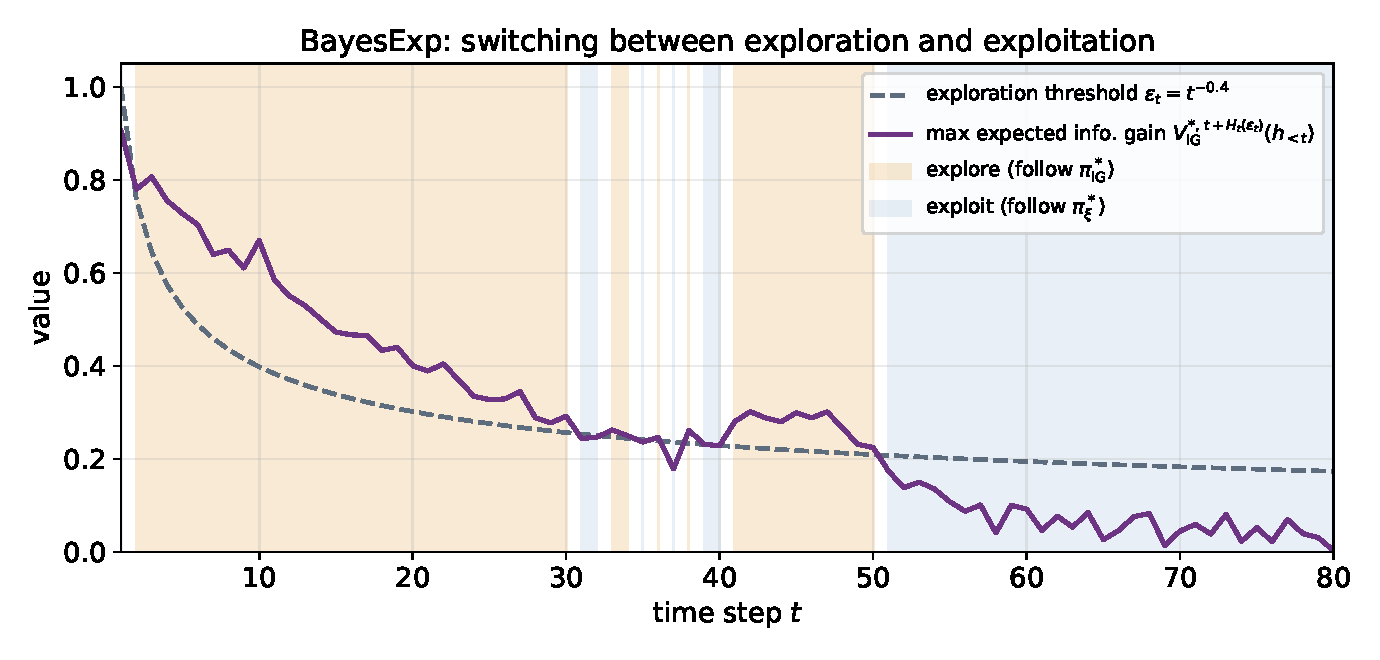
\includegraphics[width=0.75\linewidth]{bayesexp_timeline}
  \end{center}
\end{frame}

\begin{frame}{The Inquisitive Agent (Inq)}
  The \textbf{Inquisitive Reinforcement Learner (Inq)} achieves
  \textbf{strong} asymptotic optimality (Definition 8.1.7) -- optimal on
  \emph{every} run, not just on average. Similar to BayesExp, Inq combines
  Bayes-optimal $\mathrm{AI}\xi$ with the knowledge-seeking agent. But
  instead of prescribing exploration blocks deterministically, Inq follows
  maximally informative exploratory ``expeditions'' with a certain
  \emph{probability}; unlike BayesExp, these expeditions have \emph{random}
  length, possibly shorter or longer than the effective horizon.

  \vspace{0.4em}
  Also, Inq uses an \emph{undiscounted}, multi-step version of Definition
  9.3.1, and the effective horizon must be \textbf{bounded}. Otherwise Inq
  follows the same principle as BayesExp: it is more likely to explore the
  more it expects to reduce its uncertainty about which environment it is
  in. As certainty about the true environment $\mu$ grows, exploration
  becomes rarer, and asymptotically Inq converges to $\mathrm{AI}\xi$. The
  additional exploration prevents Inq from getting stuck ignorant about
  unexplored parts of the world, which guarantees it also converges to
  $\mathrm{AI}\mu$ (the Bayes-optimal agent if $\mu$ were known).

  \begin{block}{Theorem 9.4.2 (Inq is strongly asymptotically optimal [CCH19])}
    For any countable class of environments $\mathcal{M}$ and bounded
    effective horizon ($\sup_t H_t(\varepsilon)<\infty\ \forall\varepsilon>0$),
    the Inquisitive Reinforcement Learner (Inq, Algorithm 9.5) is strongly
    asymptotically optimal.
  \end{block}
\end{frame}

\begin{frame}[allowframebreaks]{Building Inq: Multi-Step Information Gain}
  First we need a multi-step generalization of the one-step ($t=n$)
  information gain from Definition 9.3.1:
  \[
    \IG_{t:n}(h_{t:n}|h_{<t}) \;:=\; \sum_{\nu\in\mathcal{M}} w(\nu|h_{1:n})\, \log\frac{w(\nu|h_{1:n})}{w(\nu|h_{<t})}
  \]
  This leads to the non-discounted truncated Information Gain Value
  function for policy $\pi$:
  \[
    V^{\pi,n}_{\IG}(h_{<t}) \;:=\; \E^\pi_\xi[\IG_{t:n}|h_{<t}] \;\equiv\; \sum_{h_{t:n}}\xi^\pi(h_{t:n}|h_{<t})\,\IG_{t:n}(h_{t:n}|h_{<t})
  \]
  and similarly to the knowledge-seeking agent, the optimal (deterministic)
  IG policy for this window is
  \[
    \pi^{*,n}_{\IG,h_{<t}} :\in \arg\max_\pi V^{\pi,n}_{\IG}(h_{<t})
  \]
  This policy is well-defined on histories from length $t-1$ up to $n$.

  \framebreak
  At each time step $t$, the action taken is
  $a_t := \pi^{*,\,t-k+m-1}_{\IG,h_{<t-k}}(h_{<t})$, for an IG policy that
  was optimized at some \emph{random} $k$ time steps earlier, with a
  \emph{random} horizon $m$. While the IG policy is (re-)sampled
  independently at each $t$, there is a non-zero chance of following the
  \emph{same} policy for $H_t(\varepsilon)$ time steps in a row, since
  $m>H_t(\varepsilon)-k$ may be sampled, and the policy that started at $t$
  may be sampled again for another $H_t(\varepsilon)$ steps. Exploring
  consistently for $H_t(\varepsilon)$ steps at a time matters -- BayesExp
  \emph{prescribes} this, Inq achieves it only with non-zero probability.

  The probability of sampling $\pi^{*,\,t-k+m-1}_{\IG,h_{<t-k}}$ is
  \[
    \varepsilon^m_k(h_{<t}) \;:=\; \min\Big\{\ \frac{1}{m^2(m+1)},\ \ \eta\, V^{\pi^{*,\,t-k+m-1}_{\IG,h_{<t-k}},\,t+m}_{\IG}(h_{<t})\ \Big\}
  \]
  for $m\in\N^+$ and $0\le k<\min\{m,t\}$, where $0<\eta<1$ (eta) is an
  exploration constant.

  \framebreak
  The first term, $1/(m^2(m+1))$, ensures the probabilities never sum to
  more than $1$: it caps how much probability mass is spent exploring for
  any particular $(k,m)$ pair, and
  \[
    \varepsilon_+(h_{<t}) \;:=\; \sum_{m\in\N^+}\sum_{k<\min\{m,t\}} \varepsilon^m_k(h_{<t}) \;\le\; \sum_{m\in\N^+}\sum_{k<m} \frac{1}{m^2(m+1)} \;=\; 1.
  \]
  The remaining probability, $1-\varepsilon_+(h_{<t})$, is used for
  following the Bayes-optimal policy $\pi^*_\xi$. Together these define
  the Inq algorithm.
\end{frame}

\begin{frame}{Algorithm 9.5: Inq}
  {\small
  \begin{algorithmic}[1]
    \Statex \textbf{Require:} Model class $\mathcal{M}$. Prior $w$. Discount $\gamma$.
    \Statex \textbf{Input:} Percept stream $e_1,e_2,e_3,\dots$
    \Statex \textbf{Output:} Action stream $a_1,a_2,a_3,\dots$
    \For{$t=1,2,3,\dots$}
      \State Take action $\pi^{*,\,t-k+m-1}_{\IG,h_{<t-k}}(h_{<t})$ with probability $\varepsilon^m_k(h_{<t})$ \Comment{exploration}
      \State Take action $\pi^*_\xi(h_{<t})$ with probability $1-\varepsilon_+(h_{<t})$ \Comment{exploitation}
    \EndFor
  \end{algorithmic}}
  \textbf{Plain English.} At every single time step, Inq flips a weighted
  coin: with the small probabilities $\varepsilon^m_k$ (summed over all
  valid $(k,m)$) it continues (or starts) an exploratory expedition guided
  by an information-gain-optimal policy computed for some window; otherwise
  (the leftover probability $1-\varepsilon_+$) it simply exploits via the
  Bayes-optimal action.
\end{frame}

\begin{frame}{Inq vs.\ BayesExp}
  \textbf{Contrast with BayesExp.} Strong asymptotic optimality may not be
  achievable for environments with (some or all) \emph{unbounded} horizon,
  since the horizon may grow faster than Inq -- or possibly any policy --
  can learn about ever-longer-term dynamics. BayesExp, by contrast, is
  \emph{weakly} asymptotically optimal even for (sublinearly) growing
  horizons. Both agents maximize information gain (explore) whenever
  enough information about the environment is expected to be gained; if
  not, they follow the Bayes-optimal agent (though calling $\pi^*_\xi$
  ``exploiting'' is not entirely fair -- $\mathrm{AI}\xi$ implicitly
  explores too, just not \emph{enough} to be asymptotically optimal on its
  own).
\end{frame}

\begin{frame}[fragile]{Python: Simulating BayesExp's Explore/Exploit Switch}
  A minimal simulation of BayesExp's decision rule, using a synthetic
  (illustrative) trace of the maximum expected information gain
  $V_{\IG}^{*}$ and the threshold schedule $\varepsilon_t=t^{-\beta}$.
  \begin{lstlisting}[style=pycode]
import numpy as np
T, beta = 20, 0.4
t = np.arange(1, T + 1)
eps_t = t ** (-beta)                 # decreasing exploration threshold

# Toy V_IG*: starts high (lots to learn), decays as the agent learns
rng = np.random.default_rng(1)
V_IG = 0.9 * np.exp(-t / 8.0) + rng.normal(0, 0.02, T)

mode = np.where(V_IG > eps_t, "EXPLORE", "exploit")
for i in range(T):
    print(f"t={t[i]:2d}  V_IG*={V_IG[i]:.3f}  eps_t={eps_t[i]:.3f}  -> {mode[i]}")
# t= 1  V_IG*=0.812  eps_t=1.000  -> exploit
# t= 2  V_IG*=0.727  eps_t=0.758  -> exploit
# t= 3  V_IG*=0.634  eps_t=0.644  -> exploit
# t= 4  V_IG*=0.577  eps_t=0.574  -> EXPLORE
# ...
# t=20  V_IG*=0.083  eps_t=0.312  -> exploit
  \end{lstlisting}
  \textbf{Observation.} Early on, when there is a lot of information to be
  gained, the agent explores; as $V_{\IG}^{*}$ decays below the shrinking
  threshold $\varepsilon_t$, BayesExp settles into exploiting the
  Bayes-optimal policy $\pi^*_\xi$ -- matching the timeline figure on the
  previous slide.
\end{frame}

%% ══════════════════════════════════════════════════════════════════════════
\section{9.5 Planning-Avoiding Agents (Self-AIXI)}

\begin{frame}{Avoiding Expensive Planning}
  Rather than explicit \textbf{expectimax planning} (which in practice is
  typically approximated by Monte Carlo Tree Search), there exist
  reinforcement-learning algorithms that side-step planning entirely by
  learning a \textbf{Q-value function} directly -- via solving Bellman
  (optimality) equations in theory, or via \textbf{Temporal Difference
  (TD)}-style algorithms in practice -- or by directly learning a policy.

  \vspace{0.4em}
  \textbf{Planning-avoiding universal agents} have also been developed. In
  this section we introduce \textbf{Self-AIXI} [CGMH+23], which
  self-predicts its own action stream. (Two related approaches: AIXI$tl$,
  Section 13.2, computes a provable lower bound to the value function;
  \emph{Compress and Control}, Section 12.9, is another way to avoid
  planning.)

  \vspace{0.4em}
  \textbf{Self-AIXI} is a universal agent using \textbf{self-prediction}
  instead of traditional planning. It generates a stream of action data
  akin to methods used by other TD(0) agents, executing a one-step action
  maximization based on current \emph{on-policy} Q-value estimates for a
  mixture-policy. Despite only performing one-step-lookahead ``planning'',
  Self-AIXI converges to the (long-horizon) Bayes-optimal $\mathrm{AI}\xi$,
  is self-optimizing, and has maximal Legg--Hutter intelligence.
\end{frame}

\begin{frame}{Definition 9.5.1: Bayesian Mixture Policy and Self-AIXI}
  Self-AIXI predicts its own stream of actions via a Bayesian mixture
  policy $\zeta$ (zeta) over a class of policies $\Pi$, in a dual fashion
  to the Bayesian mixture \emph{environment} $\xi$ over $\mathcal{M}$:
  \begin{block}{Definition 9.5.1 (Bayesian mixture policy and Self-AIXI)}
    The Bayesian mixture $\zeta$ over a countable class of policies $\Pi$
    is defined as
    \[
      \zeta(a_t|h_{<t}) \;:=\; \sum_{\pi\in\Pi} \omega(\pi|h_{<t})\,\pi(a_t|h_{<t}), \qquad
      \omega(\pi|h_{1:t}) \;:=\; \omega(\pi|h_{<t})\,\frac{\pi(a_t|h_{<t})}{\zeta(a_t|h_{<t})} \;=\; \omega_\pi\,\frac{\pi(a_{1:t}\|e_{<t})}{\zeta(a_{1:t}\|e_{<t})}
    \]
    Self-AIXI takes the one-step optimal action according to \emph{both}
    the Bayesian mixture environment $\xi$ over $\mathcal{M}$ with prior
    $w_\nu$ \emph{and} the Bayesian mixture policy $\zeta$ over $\Pi$ with
    prior $\omega(\pi|\epsilon)\equiv\omega_\pi$:
    \[
      \pi_S(h_{<t}) \;:=\; \arg\max_{a_t} Q^\zeta_\xi(h_{<t}a_t)
    \]
    where the Q-value is as in Definition 6.7.1.
  \end{block}
\end{frame}

\begin{frame}{Definition 9.5.1: Plain-English Summary}
  \textbf{Plain English.} $\omega_\pi$ (omega) is a prior weight over
  \emph{policies}, exactly analogous to $w_\nu$ over environments. $\zeta$
  is a mixture -- a weighted blend -- of many candidate policies, updated
  by Bayes' rule just like $\xi$ is updated over environments (each
  observed action $a_t$ reweights $\omega(\pi|h_{1:t})$ toward policies
  that would have predicted it).
\end{frame}

\begin{frame}{Understanding Self-AIXI's Action Rule}
  \begin{center}
    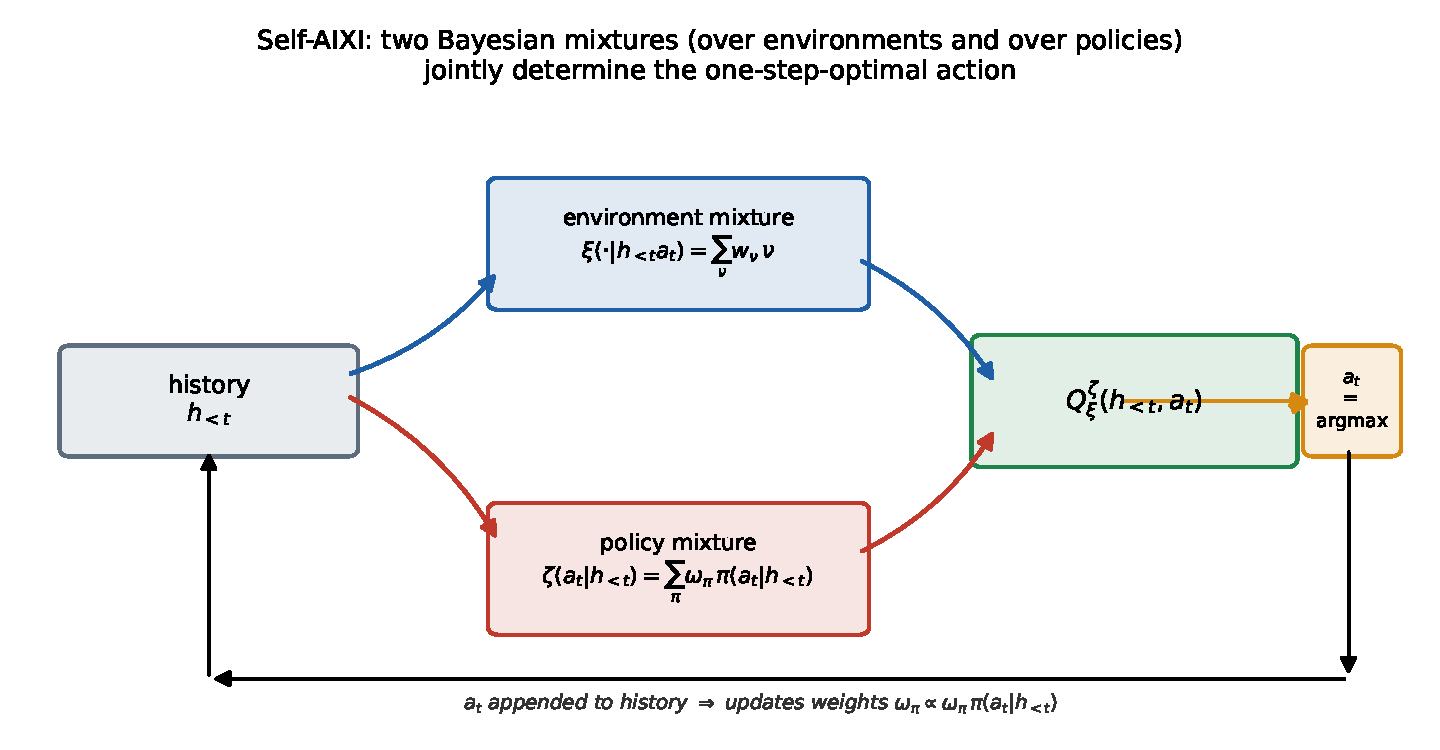
\includegraphics[width=0.85\linewidth]{selfaixi_schematic}
  \end{center}
\end{frame}

\begin{frame}{Self-AIXI: The Self-Improving Loop}
  Importantly, Self-AIXI maximizes the \textbf{Q-values from the mixture
  policy} $\zeta$ instead of the fully optimal policy $\pi^*_\xi$. This
  means there is no need to optimize over the (expensive, long-horizon)
  future: only the \emph{on-policy} Q-values of the current $\zeta$ are
  needed, which are typically far easier to estimate than the optimal
  off-policy Q-values $Q^*_\xi$.

  \vspace{0.3em}
  \textbf{Self-improving loop.} The action selected by Self-AIXI
  necessarily improves, by definition of $\arg\max$, over the current
  value estimate: $\max_{a_t}Q^\zeta_\xi(h_{<t}a_t)\ge V^\zeta_\xi(h_{<t})$.
  This action is then appended to the next history $h_{<t+1}$, which is
  in turn consumed by the policy-mixture $\zeta$ at the next time step --
  so $\zeta$ does Bayesian inference over its own, self-generated stream of
  actions, and makes progressively better action predictions over time.
  Self-AIXI is thus \emph{self-predicting} its own small, incremental
  improvements.
\end{frame}

\begin{frame}{Theorem 9.5.2: Convergence Properties of Self-AIXI}
  In the case of using the largest class of \emph{all} computable
  policies, the mixture $\zeta$ becomes a Solomonoff (action) predictor
  with enough representational power to approximate, within itself, both
  the policy evaluation \emph{and} the policy improvement operation.

  \begin{block}{Theorem 9.5.2 (Convergence properties of Self-AIXI [CGMH+23])}
    Under various conditions, the value functions of Self-AIXI $\pi_S$
    converge to those of Bayes-optimal $\mathrm{AI}\xi$ in expectation on
    histories generated by $\pi_S$ interacting with $\mu$:
    \[
      \E^{\pi_S}_\mu\big[V^{\pi_\xi^*}_\xi(h_{<t}) - V^{\pi_S}_\xi(h_{<t})\big] \xrightarrow{t\to\infty} 0,
      \qquad
      \E^{\pi_S}_\mu\big[V^{\pi_\xi^*}_\mu(h_{<t}) - V^{\pi_S}_\mu(h_{<t})\big] \xrightarrow{t\to\infty} 0
    \]
  \end{block}
  \textbf{Plain English.} Both the value \emph{Self-AIXI believes it is
  getting} (w.r.t.\ $\xi$) and the value \emph{it actually gets} (w.r.t.\
  the true $\mu$) converge to the Bayes-optimal value -- i.e.\ despite
  only ever doing one-step lookahead, Self-AIXI eventually performs as
  well as full long-horizon Bayes-optimal planning.
\end{frame}

\begin{frame}{Consequences of Theorem 9.5.2}
  This implies that for environment classes $\mathcal{M}$ admitting
  \textbf{self-optimizing} policies (Figure 7.1), since
  $\mathrm{AI}\xi$ is self-optimizing (Theorem 7.3.6), \textbf{Self-AIXI is
  too}:
  \[
    V^*_\mu(h_{<t}) - V^{\pi_S}_\mu(h_{<t}) \;\xrightarrow{t\to\infty}\; 0 \qquad \mu^\pi\text{-almost surely, for any } \pi
  \]
  For $\pi=\pi_S$, this implies $\pi_S$ is \textbf{strongly asymptotically
  optimal}. For $\mathcal{M}=\mathcal{M}_{\mathrm{sol}}$ (the class of all
  computable environments), the first convergence result implies
  Self-AIXI asymptotically has \textbf{maximal universal intelligence}
  $\Upsilon$ (Upsilon, the Legg--Hutter intelligence measure,
  Definition 16.7.1):
  \[
    \E^{\pi_S}_\mu\Big[\max_\pi \Upsilon(\pi|h_{<t}) - \Upsilon(\pi_S|h_{<t})\Big] \;\xrightarrow{t\to\infty}\; 0
  \]
  \textbf{Proof idea.} Self-AIXI initially acts like a one-step optimal
  (greedy) agent, and this shows up in the action sequence it produces.
  The mixture $\zeta$ then \emph{learns} to act like a one-step optimal
  agent, which means Self-AIXI starts acting like a \emph{two}-step
  optimal agent. This bootstrapping continues indefinitely, and the
  performance of Self-AIXI converges to that of $\mathrm{AI}\xi$.
  $\blacksquare$

  \vspace{0.4em}
  These results show that agents can perform well in the general
  reinforcement learning setting \emph{without} utilizing explicit
  planning at all. Experiments comparing Self-AIXI with MC-AIXI-CTW
  (Chapter 12) and full proofs are in [CGMH+23].
\end{frame}

\begin{frame}[fragile]{Python: A Toy Self-Prediction Loop}
  A stripped-down illustration of the self-improving loop: two candidate
  policies (mixture components) compete for weight $\omega_\pi$ as
  Self-AIXI's own actions are fed back in as data.
  \begin{lstlisting}[style=pycode]
import numpy as np
policies = {                 # toy: P(action=1 | h) for two policies
    "explore_biased": 0.7,
    "exploit_biased": 0.2,
}
omega = {"explore_biased": 0.5, "exploit_biased": 0.5}   # prior omega_pi

def zeta(a):                 # mixture policy zeta(a_t | h_<t)
    return sum(omega[p] * (policies[p] if a == 1 else 1 - policies[p])
               for p in policies)

rng = np.random.default_rng(0)
for t in range(6):
    # Self-AIXI would take a_t = argmax_a Q^zeta_xi(h,a); here we just
    # illustrate the *belief update* step after an action is produced.
    a_t = 1 if rng.random() < zeta(1) else 0
    for p in policies:
        like = policies[p] if a_t == 1 else 1 - policies[p]
        omega[p] *= like
    z = sum(omega.values()); omega = {p: v / z for p, v in omega.items()}
    e1, e2 = omega["explore_biased"], omega["exploit_biased"]
    print("t=", t, " a_t=", a_t, " omega_explore=", round(e1, 3), " omega_exploit=", round(e2, 3))
  \end{lstlisting}
\end{frame}

\begin{frame}{Self-Prediction Loop: Idea}
  \textbf{Idea.} Every self-generated action $a_t$ is Bayesian evidence
  about which policy in the mixture best explains Self-AIXI's own past
  behaviour, exactly as Definition 9.5.1's update rule for
  $\omega(\pi|h_{1:t})$ prescribes.
\end{frame}

%% ══════════════════════════════════════════════════════════════════════════
\section{9.6 Exercises}

\begin{frame}[allowframebreaks]{Exercises}
  \begin{enumerate}
    \item[\textbf{1.}] [C25] Prove Theorem 9.1.3.
    \item[\textbf{2.}] [C32] Prove Theorem 9.2.1.
    \item[\textbf{3.}] [C28] Prove Theorem 9.4.1.
    \item[\textbf{4.}] [C20] Prove that if $H_t(\varepsilon)=o(t)$, then
      there exists $\varepsilon_t\to0$ such that $H_t(\varepsilon_t)=o(t\varepsilon_t)$
      as required in Theorem 9.4.1.
    \item[\textbf{5.}] [C45o] Prove/disprove that Thompson sampling is
      weakly asymptotically optimal.
    \item[\textbf{6.}] [C45o] Prove/disprove that using Thompson sampling
      with an $\varepsilon$-optimal policy for the sampled environment
      leads to an agent which is asymptotically optimal in expectation.
    \item[\textbf{7.}] [C20i] Prove that $w_\nu=2^{-K(\nu)}$ has infinite
      entropy $\sum_{\nu\in\mathcal{M}_{\mathrm{sol}}} w_\nu\log w_\nu^{-1}$,
      but $w_\nu=2^{-(1+\varepsilon)K(\nu)}$ and $w_\nu=2^{-K(\nu)}/K(\nu)$
      have finite entropy.
    \item[\textbf{8.}] [C38] BayesExp uses explicit exploration to achieve
      weak asymptotic optimality. Bayesian agents like AIXI will still
      (implicitly) explore. Derive a definition for the kind of
      exploration a Bayesian agent does. Using this definition, find the
      largest class of environments $\mathcal{M}$ such that AIXI is
      asymptotically optimal (for each type).
    \item[\textbf{9.}] [C45o] Prove/disprove that using BayesExp with an
      $\varepsilon$-optimal policy during the exploitation (and/or
      exploration) phases leads to an agent which is weakly asymptotically
      optimal?
  \end{enumerate}
  \textbf{Reading the difficulty codes.} The bracketed code (e.g.\
  [C25], [C45o]) is the book's difficulty rating: roughly, the number
  gives an estimated difficulty out of $50$, ``C'' marks a
  \emph{creative}/research-flavoured exercise, and a trailing ``o''
  marks an \emph{open} problem without a currently known complete
  solution.
\end{frame}

%% ══════════════════════════════════════════════════════════════════════════
\section{9.7 History and References}

\begin{frame}[allowframebreaks]{History and References}
  \textbf{Optimism.} Optimism has long been an approach to the exploration
  problem in reinforcement learning [SL08]. The optimistic variant of AIXI
  and its philosophical and axiomatic underpinning were first introduced in
  [SH12b], where it was shown how optimism can lead to asymptotic
  optimality (Section 9.1). Optimism of general agents was further studied
  in the context of cognitive theory and rational behaviour [SH14a,SH15b].
  On the opposite end of the spectrum, pessimism in general reinforcement
  learning can lead to more \emph{safe} behaviour [CH20b]. A counter-point
  to optimism was presented in [OVR16b], which argued that any optimistic
  algorithm matching Thompson sampling in statistical efficiency would
  likely be computationally intractable.

  \framebreak
  \textbf{Thompson sampling.} Thompson sampling [Tho33] (Section 9.2) has
  had a recent resurgence, showing strong performance in many problems
  beyond the traditional bandit setting, including: contextual bandits
  [AG13], finite-time bandits [CPRR17], non-stationary bandits [RK17],
  MDPs [GM15,OGNJ17,OVR16a], POMDPs [JJJN21], game theory [Mau20], adaptive
  control [OB10b,OB10a,Ort11], and (general) reinforcement learning
  [LLOH16,LLOH17]. A thorough overview is given in [RVRK+17]. Using naive
  sequential prediction to solve sequential decision-making problems can
  lead to several difficulties [OKD+21]; however [OWR+19] showed how to
  \emph{meta-learn} a Thompson sampling agent and overcome many of these
  difficulties. Thompson-sampling-based exploration has been shown to
  work well in Atari when using an uncertainty-based Bellman equation
  [OOMM17].

  \framebreak
  \textbf{Knowledge-seeking agents.} The knowledge-seeking agent was first
  proposed in [Ors11] and later extended to stochastic environments in
  [OLH13] (Section 9.3). It was extended again from stochastic to
  \emph{quantum} environments in [Sar21,SAAGB21].

  \vspace{0.3em}
  \textbf{Curiosity-based agents.} Highly related to knowledge-seeking
  agents are curiosity-based agents: agents that use a notion of curiosity
  to aid exploration, or in some cases replace reward entirely. One of the
  earliest curiosity-based agents was [Sch91], incentivized to take
  actions providing more information about the environment. [BEP+18]
  studied curiosity-based agents in Atari and other RL environments. A
  known weakness of curiosity/information-seeking agents is susceptibility
  to ``noisy TVs'': any input feeding unpredictable random data to the
  agent looks endlessly informative. The original knowledge-seeking agent
  [Ors11] (which only modelled deterministic environments) suffers this
  problem. [MPYBG22] investigated how curiosity-based agents can overcome
  it. Variational Information Maximizing has been shown to be an effective
  curiosity-based exploration method [HCD+16]. [SGS11] introduced an
  exploration strategy using a curiosity-based (action) value function and
  proved its (Bayesian exploration) optimality when the environment is an
  MDP. Curiosity is not always positive for an agent, and the dangers of
  \emph{overly} curious agents were discussed in [CHC21].

  \framebreak
  \textbf{Intrinsic rewards.} One key aspect of knowledge-seeking agents is
  that they possess an \textbf{intrinsic reward}. Intrinsic motivation and
  reward has seen substantial study; [LAW+20] surveys many approaches.
  [BSC+04] studied intrinsic motivation's ability to lead to hierarchical
  learning. [Sch10] proposed a precise theory of creativity, fun, and
  intrinsic motivation, itself motivated by compression. One approach in
  the absence of rewards is to use the discovery of new behaviour in the
  form of \emph{options} [SP02] to motivate the agent [MB16]. Intrinsic
  motivation can also guide the exploration of agents [BSO+16,MBMK21]. This
  topic will see further exploration in Chapter 15.

  \framebreak
  \textbf{General exploration agents.} The BayesExp agent [LH14a] (Section
  9.4) was the first agent shown to be weakly asymptotically optimal in a
  large class of environments, demonstrating that weak asymptotic
  optimality was an \emph{achievable} property of general agents (though
  not deterministic ones). [Lei16a] introduced an exploration measure,
  called \emph{exploration potential}, provably equivalent to asymptotic
  optimality (under some conditions). The Inq agent [CCH19] was the first
  agent shown to be \emph{strongly} asymptotically optimal, demonstrating
  (with BayesExp) that strong asymptotic optimality was an achievable
  property -- previously suspected, but not proven, that no general agent
  could achieve this.

  \vspace{0.3em}
  \textbf{Planning-avoiding agents.} For finite-state MDPs, Bellman
  equations [BT96] and Temporal Difference algorithms [HL07,SB18]
  bootstrap values and policies by one-step (or few-step) lookahead
  instead of expensive (long-horizon) expectimax or Monte Carlo Tree
  Search planning. These ideas extend to infinite MDPs via (non)linear
  value function approximation and POMDPs. In this chapter we discussed
  the history-based planning-avoiding agent Self-AIXI [CGMH+23], which
  maintains a Bayesian posterior mixture over policies. Section 13.2
  discusses AIXI$tl$ [Hut05b, Chp.\,7], and Section 12.9 discusses
  Compress and Control [VBH+15,DRW+24].

  \framebreak
  \textbf{Risk- and ambiguity-sensitivity agents.} Bayes-optimal agents are
  \textbf{risk-neutral} since they attune solely to the expected return, in
  contrast to \textbf{risk-sensitive} agents, which are also sensitive to
  higher-order moments of the return. Bayes-optimal agents are also
  \textbf{ambiguity-neutral} since they act in new situations as if the
  uncertainty were known, unlike \textbf{ambiguity-sensitive} agents, which
  act differently when recognizing situations in which they lack
  knowledge. [GMDK+22] show how off-policy meta-learning can give rise to
  risk- and ambiguity-sensitive agents, which can be safer and more robust
  to external perturbations.
\end{frame}

%% ══════════════════════════════════════════════════════════════════════════
\section{Summary}

\begin{frame}{Chapter 9 Summary}
  \begin{itemize}
    \item \textbf{Optimistic agents} ($\pi^\circ$) replace Bayesian
      averaging with a best-case maximization over the still-consistent
      environment class $\mathcal{M}_t$; provably asymptotically optimal
      (Theorem 9.1.1) with an explicit finite error bound (Theorem 9.1.2),
      extending from finite deterministic classes to stochastic, countable,
      compact, and separable classes.
    \item \textbf{Thompson sampling} ($\pi_{\mathrm{TS}}$) samples one
      environment from the posterior and commits to its optimal policy for
      a while; asymptotically optimal \emph{in mean} (Theorem 9.2.1) with
      sublinear regret (Corollary 9.2.2), though not strongly
      asymptotically optimal.
    \item \textbf{Knowledge-seeking agents} ($\pi^*_{\IG}$) replace reward
      with information gain (KL divergence between successive posteriors);
      they learn on-policy (Theorem 9.3.6) \emph{and} off-policy (Theorem
      9.3.10), making them immune to poor prior choices in the long run.
    \item \textbf{BayesExp and Inq} add deliberate exploration on top of
      $\mathrm{AI}\xi$: BayesExp explores in scheduled blocks (weakly
      asymptotically optimal, Theorem 9.4.1); Inq explores randomly with
      history-dependent probability (strongly asymptotically optimal for
      bounded horizons, Theorem 9.4.2).
    \item \textbf{Self-AIXI} ($\pi_S$) avoids expensive planning by
      maximizing one-step Q-values under a self-predicting Bayesian mixture
      \emph{policy} $\zeta$, dual to the mixture \emph{environment} $\xi$;
      it converges to Bayes-optimal $\mathrm{AI}\xi$ (Theorem 9.5.2) and
      inherits maximal Legg--Hutter intelligence.
  \end{itemize}
  \vspace{0.3em}
  \centering\emph{Next: Chapter 10 turns to computable approximations of these universal agents.}
\end{frame}

\end{document}
